\chapter{HASIL DAN PEMBAHASAN}
\label{chap:4}

Pada penelitian ini dipaparkan hasil penelitian serta analisis dari model klasifikasi yang telah dibuat sesuai dengan desain sistem dan implementasi pada Bab 3. Data yang digunakan pada pengujian ini menggunakan dataset DRAC dengan data splitting yang telah dilakukan pra-pemrosesan sebelumnya.

Berikut adalah hasil yang didapatkan dari penelitian yang telah dilakukan:

\section{Hasil Penelitian}
\label{sec:41}

Metrik yang digunakan untuk menentukan performa dari model pada saat dilatih atau training adalah akurasi dan loss. Kedua metrik ini bertujuan untuk melihat kondisi model telah fit atau tidak yang dapat menyebabkan kesulitan dalam memprediksi data yang belum pernah dilihat oleh model tersebut.

Model yang digunakan pada proses pengujian ada tiga, yaitu model dengan nilai training accuracy tertinggi, model dengan nilai validasi tertinggi, dan model terakhir dalam pelatihan.

Evaluasi dari hasil penelitian ini dilakukan dengan menggunakan beberapa metriks lain yaitu precision, recall, dan F1-score. Metrik-metrik tersebut, digunakan untuk mengukur akurasi dari model yang telah dibuat.

\subsection{Hasil Pengujian Model tanpa menggunakan Penyesuaian}
\label{sec:411}

Untuk setiap model \emph{ResNet} yang digunakan akan dilakukan pelatihan sebanyak 100 epoch pada tiga kelas dataset berbeda, yaitu: \emph{non-diabetic retinopathy} (non-DR), \emph{proliferative diabetic retinopathy} (PDR), dan \emph{non-proliferative diabetic retinopathy} (NPDR).

Data akan diambil dari model dengan nilai training terbaik (\emph{best trained}), validasi terbaik (\emph{best validated}), serta model terakhir yang dilatih (\emph{last trained}).

Sebagai kontrol, dilakukan uji coba \emph{training} yang tidak menggunakan penyesuaian \emph{gradient-weighted class activation mapping} pada dataset sesuai pada bagian \ref{sec:32}. Uji coba ini dilakukan pada seluruh variasi model \emph{ResNet} yang digunakan dan sebagai metrik akan digunakan nilai akurasi, precision, recall, dan nilai F1.

Dikarenakan dataset yang dipakai cenderung kecil, dan data untuk testing tidak memiliki label, maka dilakukan satu parameter lain untuk penilaian, yaitu \emph{Quadratic Weighted Kappa} (QWK). Penilaian ini bertujuan untuk meninjau kesetujuan antara model yang didapatkan, dengan model yang ada pada challenge dari DRAC. Hasil pengujian metrik dapat dihilat lebih jelas pada Tabel 4.1, Tabel 4.2, dan Tabel 4.3

\pagebreak

\begin{table}[hbtp]
	\begin{center}
		\caption{Hasil Best Trained model}
		\label{tb:HasilTrainDefault}
		\begin{tabular}{|c|l|c|l|l|l|c|}
			\hline
			\rowcolor[HTML]{C0C0C0} 
			Arsitektur & \multicolumn{1}{c|}{\cellcolor[HTML]{C0C0C0}class} & acc                      & \multicolumn{1}{c|}{\cellcolor[HTML]{C0C0C0}prec} & \multicolumn{1}{c|}{\cellcolor[HTML]{C0C0C0}rec} & \multicolumn{1}{c|}{\cellcolor[HTML]{C0C0C0}F1} & QWK                                  \\ \hline
			& non-DR                                             &                          & 0,875                                             & 0,848485                                         & 0,861538                                        &                                      \\ \cline{2-2} \cline{4-6}
			& NPDR                                               &                          & 0,645833                                          & 0,72093                                          & 0,681319                                        &                                      \\ \cline{2-2} \cline{4-6}
			\multirow{-3}{*}{ResNet-18}  & PDR                                                & \multirow{-3}{*}{0,7642} & 0,636364                                          & 0,5                                              & 0,56                                            & \multirow{-3}{*}{\textbf{0.7583626695732866}} \\ \hline
			& non-DR                                             &                          & 0,83871                                           & 0,787879                                         & 0,8125                                          &                                      \\ \cline{2-2} \cline{4-6}
			& NPDR                                               &                          & 0,64                                              & 0,744186                                         & 0,688172                                        &                                      \\ \cline{2-2} \cline{4-6}
			\multirow{-3}{*}{ResNet-34}  & PDR                                                & \multirow{-3}{*}{0,748}  & 0,727273                                          & 0,571429                                         & 0,64                                            & \multirow{-3}{*}{0.7218079395196282} \\ \hline
			& non-DR                                             &                          & 0,863636                                          & 0,863636                                         & 0,863636                                        &                                      \\ \cline{2-2} \cline{4-6}
			& NPDR                                               &                          & \textbf{0,688889}                                          & 0,72093                                          & 0,704545                                        &                                      \\ \cline{2-2} \cline{4-6}
			\multirow{-3}{*}{ResNet-50}  & PDR                                                & \multirow{-3}{*}{0,7805} & 0,666667                                          & 0,571429                                         & 0,615385                                        & \multirow{-3}{*}{0.7266403960229424} \\ \hline
			& non-DR                                             &                          & 0,873016                                          & 0,833333                                         & 0,852713                                        &                                      \\ \cline{2-2} \cline{4-6}
			& NPDR                                               &                          & 0,673913                                          & 0,72093                                          & 0,696629                                        &                                      \\ \cline{2-2} \cline{4-6}
			\multirow{-3}{*}{ResNet-101} & PDR                                                & \multirow{-3}{*}{0,7805} & 0,714286                                          & \textbf{0,714286}                                         & \textbf{0,714286}                                        & \multirow{-3}{*}{0.7503614091151183} \\ \hline
			& non-DR                                             &                          & \textbf{0,878788}                                          & \textbf{0,878788}                                         & \textbf{0,878788}                                        &                                      \\ \cline{2-2} \cline{4-6}
			& NPDR                                               &                          & 0,68                                              & \textbf{0,790698}                                         & \textbf{0,731183}                                        &                                      \\ \cline{2-2} \cline{4-6}
			\multirow{-3}{*}{ResNet-152} & PDR                                                & \multirow{-3}{*}{\textbf{0,7967}} & \textbf{0,857143}                                          & 0,428571                                         & 0,571429                                        & \multirow{-3}{*}{0.6937048139657909} \\ \hline
		\end{tabular}
	\end{center}
\end{table}

Dari model dengan nilai training terbaik didapatkan nilai akurasi terbaik sebesar \textbf{0.7967} dari arsitektur \emph{ResNet-152}.

\begin{itemize}

\item Untuk dataset non-DR didapatkan nilai precision, recall, dan F1 sebesar \textbf{0.878788} dari arsitektur \emph{ResNet-152};

\item Untuk dataset NPDR didapatkan nilai precision sebesar \textbf{0.688889} dari arsitektur \emph{ResNet-50}, nilai recall sebesar \textbf{0.790698} dari arsitektur \emph{ResNet-152}, nilai F1 sebesar \textbf{0.731183} dari arsitektur \emph{ResNet-152};

\item Untuk dataset PDR didapatkan nilai precision sebesar \textbf{0.857143} dari arsitektur \emph{ResNet-152}, nilai recall sebesar \textbf{0.714286} dari arsitektur \emph{ResNet-101}, nilai F1 sebesar \textbf{0.714286} dari arsitektur \emph{ResNet-101}.

\end{itemize}

Dari seluruh arsitektur \emph{ResNet} yang digunakan, nilai QWK tertinggi sebesar \textbf{0.7583626695732866} didapatkan dari arsitektur \emph{ResNet-18}. Untuk hasil dari best validated model dari setiap arsitektur ResNet dapat dilihat pada tabel \ref{tb:HasilValDefault}

\pagebreak

\begin{table}[hbtp]
	\begin{center}
		\caption{Hasil Best Validated model}
		\label{tb:HasilValDefault}
		\begin{tabular}{|c|l|c|l|l|l|c|}
			\hline
			\rowcolor[HTML]{C0C0C0} 
			Arsitektur & \multicolumn{1}{c|}{\cellcolor[HTML]{C0C0C0}class} & acc                      & \multicolumn{1}{c|}{\cellcolor[HTML]{C0C0C0}prec} & \multicolumn{1}{c|}{\cellcolor[HTML]{C0C0C0}rec} & \multicolumn{1}{c|}{\cellcolor[HTML]{C0C0C0}F1} & QWK                                  \\ \hline
			& non-DR                                             &                          & 0,904762                                          & 0,863636                                         & 0,883721                                        &                                      \\ \cline{2-2} \cline{4-6}
			& NPDR                                               &                          & 0,698113                                          & 0,860465                                         & \textbf{0,770833}                               &                                      \\ \cline{2-2} \cline{4-6}
			\multirow{-3}{*}{ResNet-18}  & PDR                                                & \multirow{-3}{*}{0,8211} & 1                                                 & 0,5                                              & 0,666667                                        & \multirow{-3}{*}{0.7332556875533816} \\ \hline
			& non-DR                                             &                          & 0,818182                                          & \textbf{0,954545}                                & 0,881119                                        &                                      \\ \cline{2-2} \cline{4-6}
			& NPDR                                               &                          & \textbf{0,756757}                                 & 0,651163                                         & 0,7                                             &                                      \\ \cline{2-2} \cline{4-6}
			\multirow{-3}{*}{ResNet-34}  & PDR                                                & \multirow{-3}{*}{0,8049} & 0,888889                                          & \textbf{0,571429}                                & \textbf{0,695652}                                        & \multirow{-3}{*}{0.7074309213982319} \\ \hline
			& non-DR                                             &                          & 0,847222                                          & 0,924242                                         & 0,884058                                        &                                      \\ \cline{2-2} \cline{4-6}
			& NPDR                                               &                          & 0,714286                                          & 0,697674                                         & 0,705882                                        &                                      \\ \cline{2-2} \cline{4-6}
			\multirow{-3}{*}{ResNet-50}  & PDR                                                & \multirow{-3}{*}{0,7967} & 0,777778                                          & 0,5                                              & 0,608696                                        & \multirow{-3}{*}{0.7051400702187358} \\ \hline
			& non-DR                                             &                          & \textbf{0,931034}                                 & 0,818182                                         & 0,870968                                        &                                      \\ \cline{2-2} \cline{4-6}
			& NPDR                                               &                          & 0,666667                                          & \textbf{0,883721}                                & 0,76                                            &                                      \\ \cline{2-2} \cline{4-6}
			\multirow{-3}{*}{ResNet-101} & PDR                                                & \multirow{-3}{*}{0,8049} & 0,875                                             & 0,5                                              & 0,636364                                        & \multirow{-3}{*}{0.6899458931486075} \\ \hline
			& non-DR                                             &                          & 0,869565                                          & 0,909091                                         & \textbf{0,888889}                               &                                      \\ \cline{2-2} \cline{4-6}
			& NPDR                                               &                          & 0,717391                                          & 0,767442                                         & 0,741573                                        &                                      \\ \cline{2-2} \cline{4-6}
			\multirow{-3}{*}{ResNet-152} & PDR                                                & \multirow{-3}{*}{0,813}  & 0,875                                             & 0,5                                              & 0,636364                                        & \multirow{-3}{*}{0.7303200133655321} \\ \hline
		\end{tabular}
	\end{center}
\end{table}

Dari model terakhir yang telah dilatih, arsitektur \emph{ResNet-101} dan \emph{ResNet-34} mendapatkan nilai akurasi yang sama, yaitu sebesar \textbf{0.8049}.

\begin{itemize}
	
	\item Untuk dataset non-DR didapatkan nilai precision sebesar \textbf{0,931034} dari arsitektur \emph{ResNet-101}, recall sebesar \textbf{0,954545} dari arsitektur \emph{ResNet-34}, dan F1 sebesar \textbf{0,888889} dari arsitektur \emph{ResNet-152};
	
	\item Untuk dataset NPDR didapatkan nilai precision sebesar \textbf{0,756757} dari arsitektur \emph{ResNet-34}, nilai recall sebesar \textbf{0,883721} dari arsitektur \emph{ResNet-101}, nilai F1 sebesar \textbf{0,770833} dari arsitektur \emph{ResNet-18};
	
	\item Untuk dataset PDR didapatkan nilai precision sebesar \textbf{1} dari arsitektur \emph{ResNet-34}, nilai recall sebesar \textbf{0.571429} dari arsitektur \emph{ResNet-18}, nilai F1 sebesar \textbf{0,695652} dari arsitektur \emph{ResNet-34}.
	
\end{itemize}

Dari seluruh arsitektur \emph{ResNet} yang digunakan, nilai QWK tertinggi sebesar \textbf{0.7332556875533816} didapatkan dari arsitektur \emph{ResNet-18}. Untuk hasil dari model epoch terakhir dari setiap arsitektur ResNet dapat dilihat pada tabel \ref{tb:HasilLastDefault}
\pagebreak

\begin{table}[hbtp]
	\begin{center}
		\caption{Hasil Last trained model}
		\label{tb:HasilLastDefault}
		\begin{tabular}{|c|l|c|l|l|l|c|}
			\hline
			\rowcolor[HTML]{C0C0C0} 
			Arsitektur   & \multicolumn{1}{c|}{\cellcolor[HTML]{C0C0C0}class} & acc                      & \multicolumn{1}{c|}{\cellcolor[HTML]{C0C0C0}prec} & \multicolumn{1}{c|}{\cellcolor[HTML]{C0C0C0}rec} & \multicolumn{1}{c|}{\cellcolor[HTML]{C0C0C0}F1} & QWK                                  \\ \hline
			& non-DR                                             &                          & 0,861538                                          & 0,848485                                         & 0,854962                                        &                                      \\ \cline{2-2} \cline{4-6}
			& NPDR                                               &                          & 0,652174                                          & 0,697674                                         & 0,674157                                        &                                      \\ \cline{2-2} \cline{4-6}
			\multirow{-3}{*}{ResNet-18}  & PDR                                                & \multirow{-3}{*}{0,7642} & 0,666667                                          & \textbf{0,571429}                                         & \textbf{0,615385}                                        & \multirow{-3}{*}{\textbf{0.7543612091028568}} \\ \hline
			& non-DR                                             &                          & 0,857143                                          & 0,818182                                         & 0,837209                                        &                                      \\ \cline{2-2} \cline{4-6}
			& NPDR                                               &                          & 0,666667                                          & \textbf{0,790698}                                         & 0,723404                                        &                                      \\ \cline{2-2} \cline{4-6}
			\multirow{-3}{*}{ResNet-34}  & PDR                                                & \multirow{-3}{*}{0,7724} & \textbf{0,777778}                                          & 0,5                                              & 0,608696                                        & \multirow{-3}{*}{0.7289056625189767} \\ \hline
			& non-DR                                             &                          & 0,808824                                          & 0,833333                                         & 0,820896                                        &                                      \\ \cline{2-2} \cline{4-6}
			& NPDR                                               &                          & 0,581395                                          & 0,581395                                         & 0,581395                                        &                                      \\ \cline{2-2} \cline{4-6}
			\multirow{-3}{*}{ResNet-50}  & PDR                                                & \multirow{-3}{*}{0,6992} & 0,5                                               & 0,428571                                         & 0,461538                                        & \multirow{-3}{*}{0.7282307517601635} \\ \hline
			& non-DR                                             &                          & \textbf{0,909091}                                          & \textbf{0,909091}                                         & \textbf{0,909091}                                        &                                      \\ \cline{2-2} \cline{4-6}
			& NPDR                                               &                          & \textbf{0,711111}                                          & 0,744186                                         & \textbf{0,727273}                                        &                                      \\ \cline{2-2} \cline{4-6}
			\multirow{-3}{*}{ResNet-101} & PDR                                                & \multirow{-3}{*}{\textbf{0,8049}} & 0,583333                                          & 0,5                                              & 0,538462                                        & \multirow{-3}{*}{0.7417574983086521} \\ \hline
			& non-DR                                             &                          & 0,852459                                          & 0,787879                                         & 0,818898                                        &                                      \\ \cline{2-2} \cline{4-6}
			& NPDR                                               &                          & 0,603774                                          & 0,744186                                         & 0,666667                                        &                                      \\ \cline{2-2} \cline{4-6}
			\multirow{-3}{*}{ResNet-152} & PDR                                                & \multirow{-3}{*}{0,7398} & \textbf{0,777778}                                          & 0,5                                              & 0,608696                                        & \multirow{-3}{*}{0.6850781547845979} \\ \hline
		\end{tabular}
	\end{center}
\end{table}

Dari model terakhir yang telah dilatih, didapatkan nilai akurasi terbaik sebesar \textbf{0.8049} dari arsitektur \emph{ResNet-101}.

\begin{itemize}
	
	\item Untuk dataset non-DR didapatkan nilai precision, recall, dan F1 sebesar \textbf{0.909091} dari arsitektur \emph{ResNet-101};
	
	\item Untuk dataset NPDR didapatkan nilai precision sebesar \textbf{0.711111} dari arsitektur \emph{ResNet-101}, nilai recall sebesar \textbf{0.790698} dari arsitektur \emph{ResNet-34}, nilai F1 sebesar \textbf{0.727273} dari arsitektur \emph{ResNet-101};
	
	\item Untuk dataset PDR didapatkan nilai precision sebesar \textbf{0.777778} dari arsitektur \emph{ResNet-34} dan \emph{ResNet-152}, nilai recall sebesar \textbf{0.571429} dari arsitektur \emph{ResNet-18}, nilai F1 sebesar \textbf{0.615385} dari arsitektur \emph{ResNet-18}.
	
\end{itemize}

Dari seluruh arsitektur \emph{ResNet} yang digunakan, nilai QWK tertinggi sebesar \textbf{0.7543612091028568} didapatkan dari arsitektur \emph{ResNet-18}.

Grafik dari \emph{training loss}, \emph{training accuracy}, dan \emph{validation accuracy} pada setiap arsitektur yang tidak menggunakan penyesuaian \emph{class weight} dapat dilihat dengan lebih jelas pada Gambar \ref{Fig:GraphTrainingDefPt2} Nilai loss cukup tinggi pada permulaan dikarenakan ukuran \emph{batch} yang cukup kecil, sehingga jumlah training sample yang digunakan dalam satu batch untuk satu iterasi juga kecil. Namun, setelah epoch tertentu, model akan menjaga nilai loss-nya tetap stabil pada nilai yang relatif rendah.
\pagebreak
\begin{figure}[hbtp]
	\centering
	\subfloat[\centering Training Loss dan Akurasi ResNet-18]{{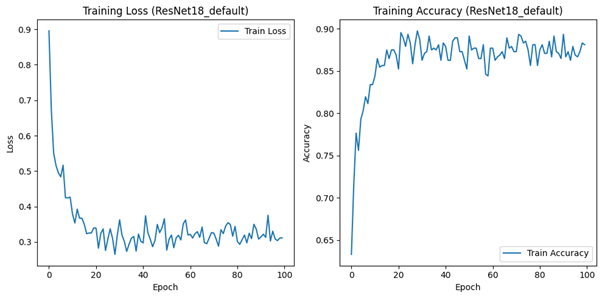
\includegraphics[height=7cm]{gambar/TrainingGraphResNet18.png}}}
	\qquad
	\subfloat[\centering Training Loss dan Akurasi ResNet-34]{{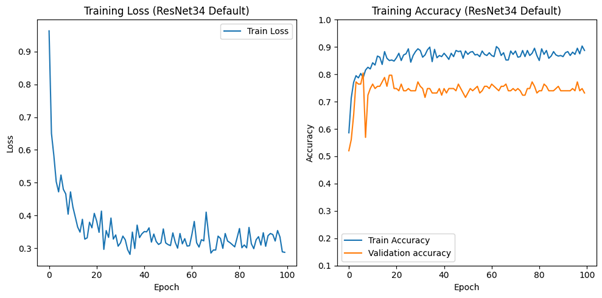
\includegraphics[height=7cm]{gambar/TrainingGraphResNet34.png}}}
	\caption{Grafik Training Loss dan akurasi ResNet-18 dan ResNet-34 Tanpa Penyesuaian Beban pada \emph{Class}}
	\label{Fig:GraphTrainingDefPt1}
\end{figure}

Dari grafik Training Loss dari \emph{ResNet-18 Default} dan \emph{ResNet-34 Default}  dapat dilihat bahwa nilai loss mulai dari \textbf{1.0}/mendekati \textbf{1.0} dan dengan cepat menjadi stabil mendekati epoch ke-\textbf{20} dengan nilai menjadi fluktuatif di antara \textbf{0.3 dan 0.4}.

Dari grafik Training Accuracy \emph{ResNet-18 Default} dapat dilihat bahwa akurasi training mulai dari nilai \textbf{0.6} dan dengan cepat menjadi stabil mendekati epoch ke-\textbf{10} dimana nilai berada di antara \textbf{0.8 dan 0.9} 

Dari grafik Training Accuracy \emph{ResNet-18 Default} dapat dilihat bahwa akurasi validasi mulai dari nilai \textbf{0.6} dan bersifat fluktuatif hingga epoch ke-\textbf{20} dimana nilai menjadi stabil di antara \textbf{0.7 dan 0.8}.

Dari grafik Training Accuracy \emph{ResNet-34 Default} dapat dilihat bahwa akurasi validasi mulai dari nilai \textbf{0.5} dan bersifat fluktuatif hingga sebelum epoch ke-\textbf{20} dimana nilai menjadi stabil di antara \textbf{0.7 dan 0.8}.

Untuk Grafik training ResNet-50 dan Resnet-101, dapat dilihat pada Gambar \ref{Fig:GraphTrainingDefPt2} di bawah ini.

\begin{figure}[hbtp]
	\centering
	\subfloat[\centering Training Loss dan Akurasi ResNet-50]{{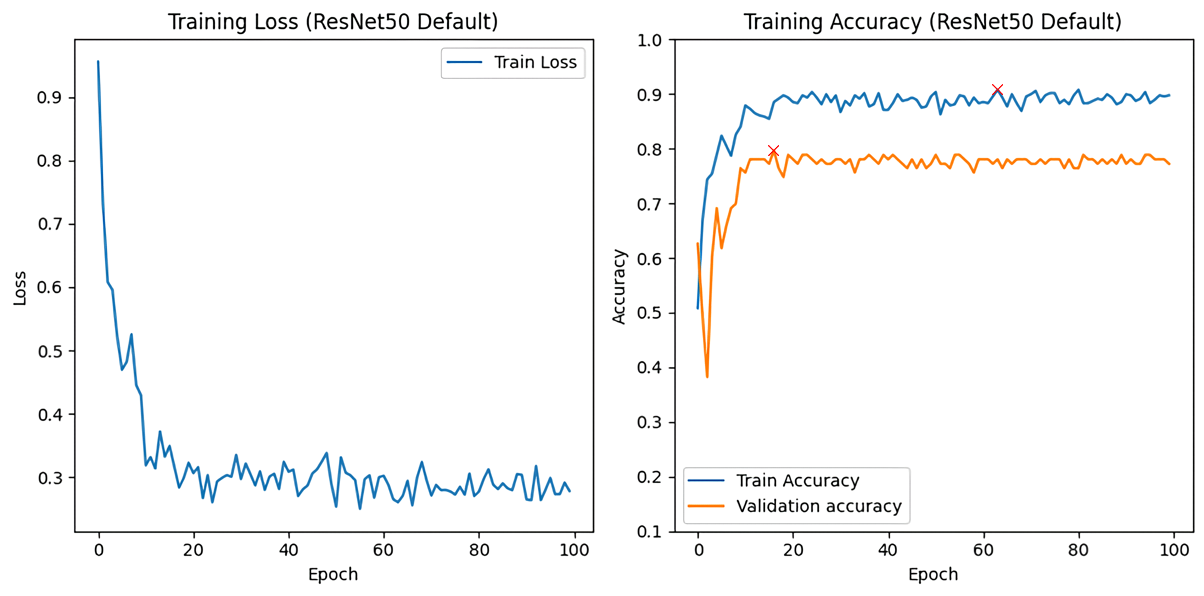
\includegraphics[height=7cm]{gambar/TrainingGraphResNet50.png}}}
	\qquad
	\subfloat[\centering Training Loss dan Akurasi ResNet-101]{{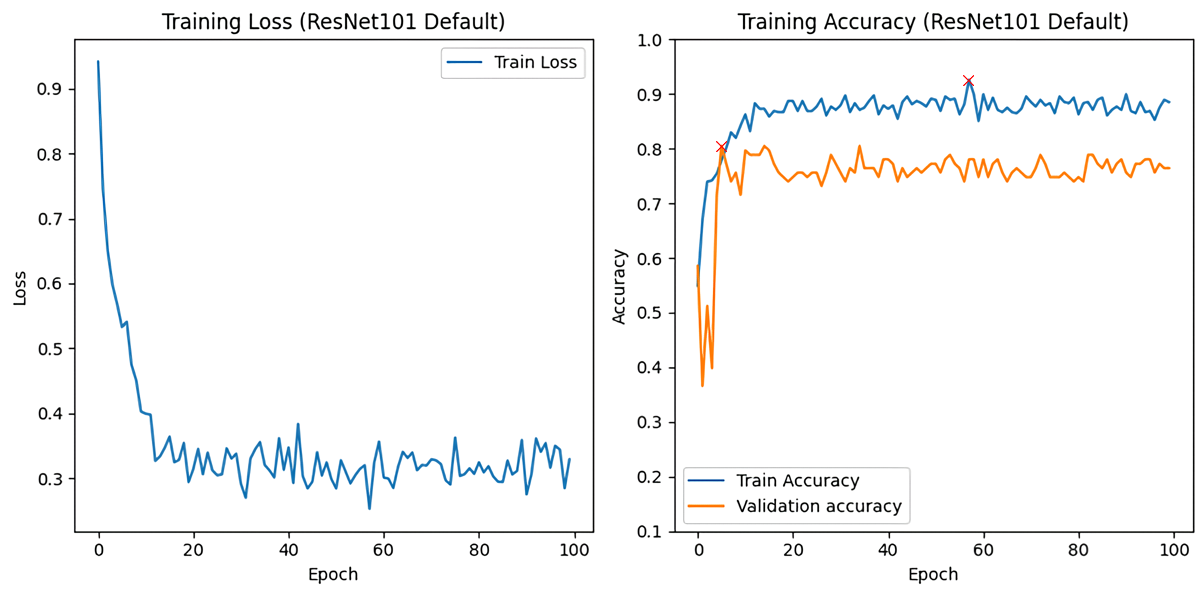
\includegraphics[height=7cm]{gambar/TrainingGraphResNet101.png}}}
	\caption{Grafik Training Loss dan akurasi ResNet-50 dan ResNet-101 Tanpa Penyesuaian Beban pada \emph{Class}}
	\label{Fig:GraphTrainingDefPt2}
\end{figure}
Dari grafik Training Loss \emph{ResNet-50 Default} dapat dilihat bahwa nilai loss mulai dari \textbf{1.0} dan dengan cepat menjadi stabil mendekati epoch ke-\textbf{20} dengan nilai menjadi fluktuatif di antara \textbf{0.3 dan 0.4}.

Dari grafik Training Accuracy \emph{ResNet-50 Default} dapat dilihat bahwa akurasi training mulai dari nilai \textbf{0.6} dan dengan cepat menjadi stabil mendekati epoch ke-\textbf{10} dimana nilai berada di antara \textbf{0.8 dan 0.9} 

Dari grafik Training Accuracy \emph{ResNet-50 Default} dapat dilihat bahwa akurasi validasi mulai dari nilai \textbf{0.6} dan bersifat fluktuatif hingga epoch ke-\textbf{20} dimana nilai menjadi stabil di antara \textbf{0.7 dan 0.8}.

Kemudian Dari grafik Training Loss \emph{ResNet-101 Default} dapat dilihat bahwa nilai loss mulai dari \textbf{1.0} dan dengan cepat menjadi stabil mendekati epoch ke-\textbf{20} dengan nilai menjadi fluktuatif di antara \textbf{0.3 dan 0.4}.

Dari grafik Training Accuracy \emph{ResNet-101 Default} dapat dilihat bahwa akurasi training mulai dari nilai \textbf{0.6} dan dengan cepat menjadi stabil mendekati epoch ke-\textbf{10} dimana nilai berada di antara \textbf{0.8 dan 0.9} 

Dari grafik Training Accuracy \emph{ResNet-101 Default} dapat dilihat bahwa akurasi validasi mulai dari nilai \textbf{0.6} dan bersifat fluktuatif hingga epoch ke-\textbf{20} dimana nilai menjadi stabil di antara \textbf{0.7 dan 0.8}.

\begin{figure}[hbtp]
	\subfloat[\centering Training Loss dan Akurasi ResNet-152]{{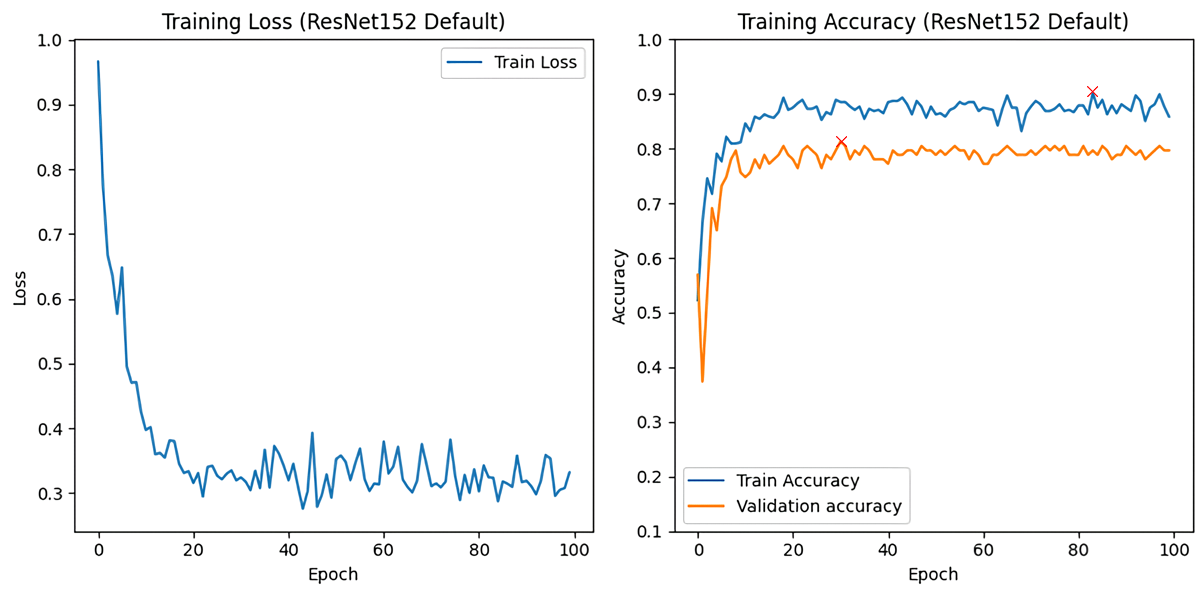
\includegraphics[height=7cm]{gambar/TrainingGraphResNet152.png}}}
	\caption{Grafik Training Loss dan akurasi ResNet-152 Tanpa Penyesuaian Beban pada \emph{Class}}
	\label{Fig:GraphTrainingDefPt3}
\end{figure}
Dari grafik Training Loss \emph{ResNet-152 Default} dapat dilihat bahwa nilai loss mulai dari \textbf{1.0} dan dengan cepat menjadi stabil mendekati epoch ke-\textbf{20} dengan nilai menjadi fluktuatif di antara \textbf{0.3 dan 0.4}.

Dari grafik Training Accuracy \emph{ResNet-152 Default} dapat dilihat bahwa akurasi training mulai dari nilai \textbf{0.6} dan dengan cepat menjadi stabil mendekati epoch ke-\textbf{10} dimana nilai berada di antara \textbf{0.8 dan 0.9} 

Dari grafik Training Accuracy \emph{ResNet-152 Default} dapat dilihat bahwa akurasi validasi mulai dari nilai \textbf{0.6} dan bersifat fluktuatif hingga epoch ke-\textbf{20} dimana nilai menjadi stabil di antara \textbf{0.7 dan 0.8}.

Untuk \emph{confusion matrix} dari setiap arsitektur dapat dilihat pada Gambar \ref{fig:confRes18}, Gambar \ref{fig:confRes34}, Gambar \ref{fig:confRes50}, Gambar \ref{fig:confRes101}, dan Gambar \ref{fig:confRes152}. Masing - masing gambar terdiri dari tiga \emph{confusion matrix}, yang merupakan hasil dari model terbaik pada akurasi \emph{training}, model terbaik pada akurasi validasi, dan model terakhir dari 100 \emph{epoch} pada arsitektur tersebut.
\pagebreak
\begin{figure}[hbtp]
	\centering
	\subfloat[\centering Best Train acc ResNet-18]{{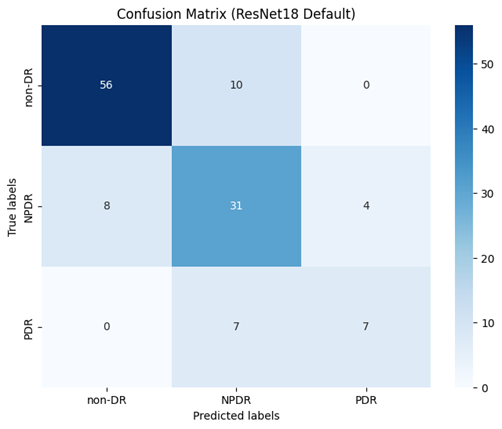
\includegraphics[width=7cm]{gambar/confusionMatrixResnet18_bestTrain.png} }}%
	\qquad
	\subfloat[\centering Best Val acc ResNet-18]{{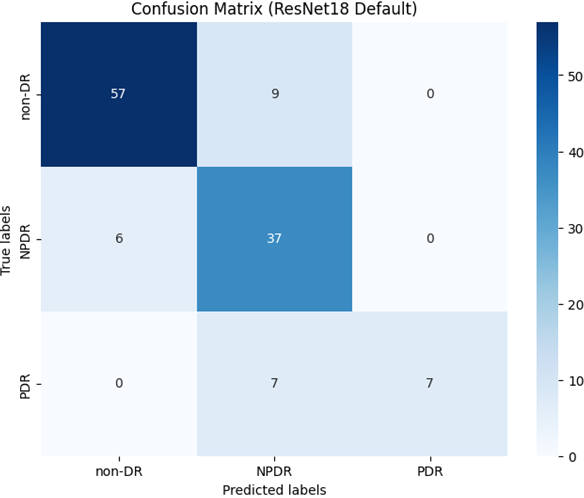
\includegraphics[width=7cm]{gambar/confusionMatrixResnet18_bestVal.png} }}%
	\qquad
	\subfloat[\centering Last Trained ResNet-18]{{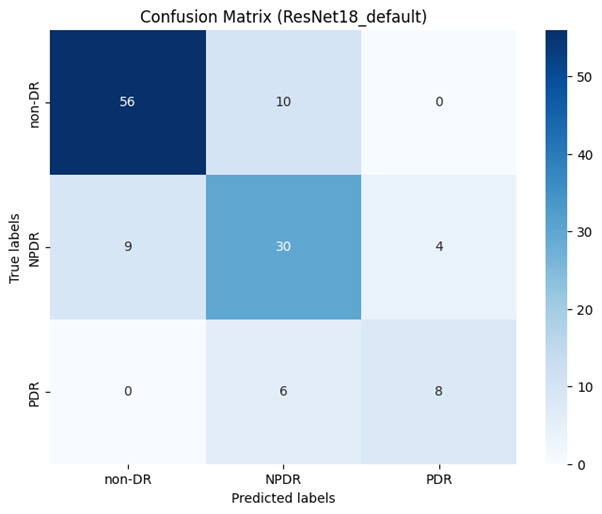
\includegraphics[width=7cm]{gambar/last model/confusionMatrixResnet18.png} }}%
	\caption{Confusion Matrix ResNet-18 yang Tidak Dilakukan Penyesuaian Beban Kelas}
	\label{fig:confRes18}
\end{figure}

\begin{itemize}
	\item Untuk dataset non-DR dapat dilihat bahwa model dapat melakukan prediksi \textbf{57 kasus non-DR} dengan akurat, dan 9 kasus diprediksi salah sebagai NDPR tanpa prediksi untuk PDR.
	
	\item Untuk dataset NPDR dapat dilihat bahwa model dapat melakukan prediksi \textbf{37 kasus NPDR} dengan akurat, dan 6 kasus diprediksi sebagai non-DR tanpa prediksi untuk PDR.
	
	\item Untuk dataset PDR dapat dilihat bahwa model dapat melakukan prediksi \textbf{8 kasus PDR} dengan akurat, dan 6 kasus diprediksi sebagai NPDR tanpa prediksi non-DR.
\end{itemize}
\pagebreak

\begin{figure}[hbtp]
	\centering
	\subfloat[\centering Best Train acc ResNet-34]{{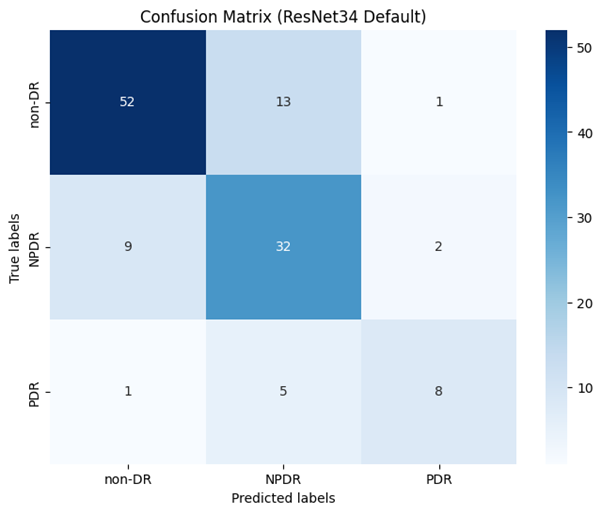
\includegraphics[width=7cm]{gambar/confusionMatrixResnet34_bestTrain.png} }}%
	\qquad
	\subfloat[\centering Best Val acc ResNet-34]{{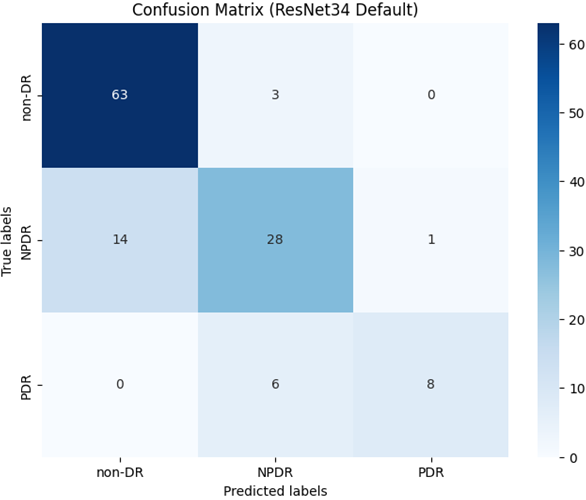
\includegraphics[width=7cm]{gambar/confusionMatrixResnet34_bestVal.png} }}%
	\qquad
	\subfloat[\centering Last Trained ResNet-34]{{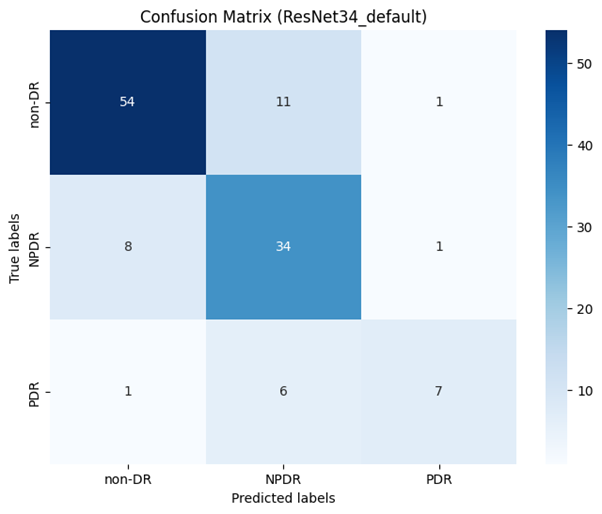
\includegraphics[width=7cm]{gambar/last model/confusionMatrixResnet34.png} }}%
	\caption{Confusion Matrix ResNet-34 yang Tidak Dilakukan Penyesuaian Beban Kelas}
	\label{fig:confRes34}
\end{figure}

\begin{itemize}
	\item Untuk dataset non-DR dapat dilihat bahwa model dapat melakukan prediksi \textbf{63 kasus non-DR} dengan akurat, dan 3 kasus diprediksi salah sebagai NDPR tanpa prediksi untuk PDR.
	
	\item Untuk dataset NPDR dapat dilihat bahwa model dapat melakukan prediksi \textbf{34 kasus NPDR} dengan akurat, 8 kasus diprediksi sebagai non-DR, dan 1 kasus diprediksi sebagai PDR.
	
	\item Untuk dataset PDR dapat dilihat bahwa model dapat melakukan prediksi \textbf{8 kasus PDR} dengan akurat, dan 6 kasus diprediksi sebagai NPDR tanpa prediksi non-DR.
\end{itemize}
\pagebreak

\begin{figure}[hbtp]
	\centering
	\subfloat[\centering Best Train acc ResNet-50]{{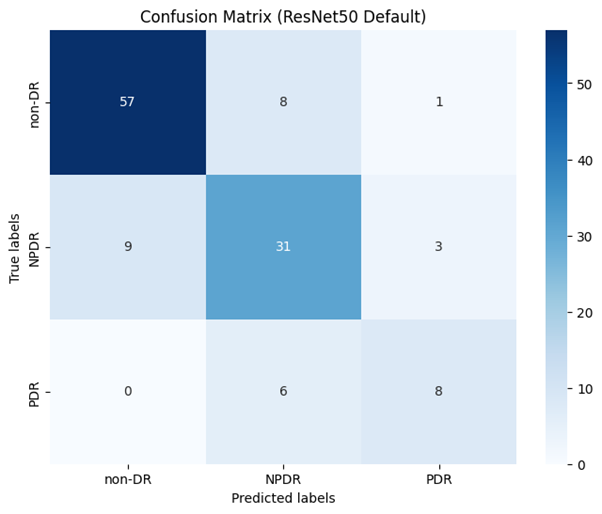
\includegraphics[width=7cm]{gambar/confusionMatrixResnet50_bestTrain.png} }}%
	\qquad
	\subfloat[\centering Best Val acc ResNet-50]{{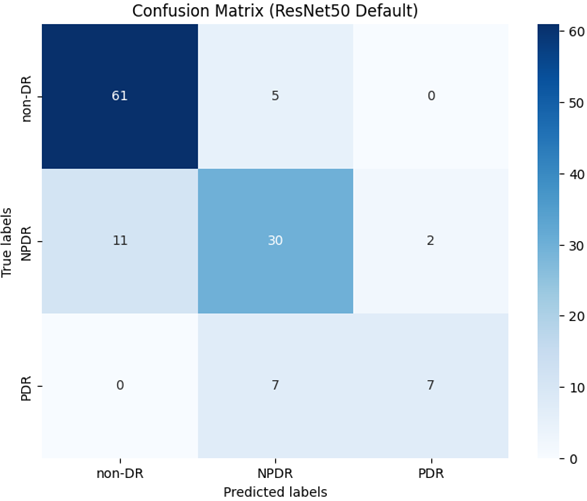
\includegraphics[width=7cm]{gambar/confusionMatrixResnet50_bestVal.png} }}%
	\qquad
	\subfloat[\centering Last Trained ResNet-50]{{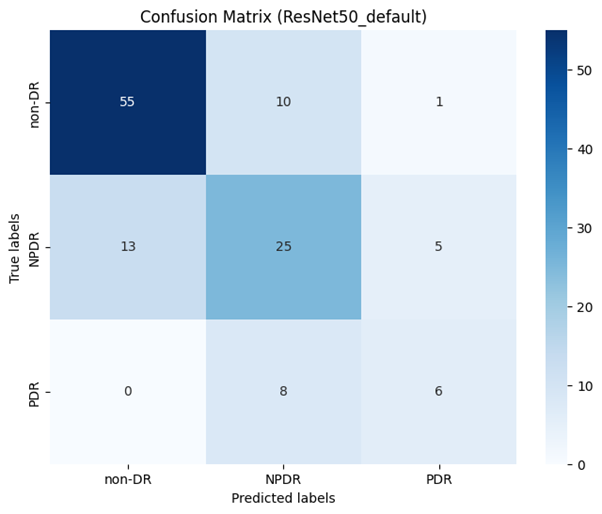
\includegraphics[width=7cm]{gambar/last model/confusionMatrixResnet50.png} }}%
	\caption{Confusion Matrix ResNet-50 Default yang Tidak Dilakukan Penyesuaian Beban Kelas}
	\label{fig:confRes50}
\end{figure}

\begin{itemize}
	\item Untuk dataset non-DR dapat dilihat bahwa model dapat melakukan prediksi \textbf{61 kasus non-DR} dengan akurat, dan 5 kasus diprediksi salah sebagai NDPR tanpa prediksi untuk PDR.
	
	\item Untuk dataset NPDR dapat dilihat bahwa model dapat melakukan prediksi \textbf{31 kasus NPDR} dengan akurat, 9 kasus diprediksi sebagai non-DR, dan 3 kasus diprediksi sebagai PDR.
	
	\item Untuk dataset PDR dapat dilihat bahwa model dapat melakukan prediksi \textbf{8 kasus PDR} dengan akurat, dan 6 kasus diprediksi sebagai NPDR tanpa prediksi non-DR.
\end{itemize}
\pagebreak

\begin{figure}[hbtp]
	\centering
	\subfloat[\centering Best Train acc ResNet-101]{{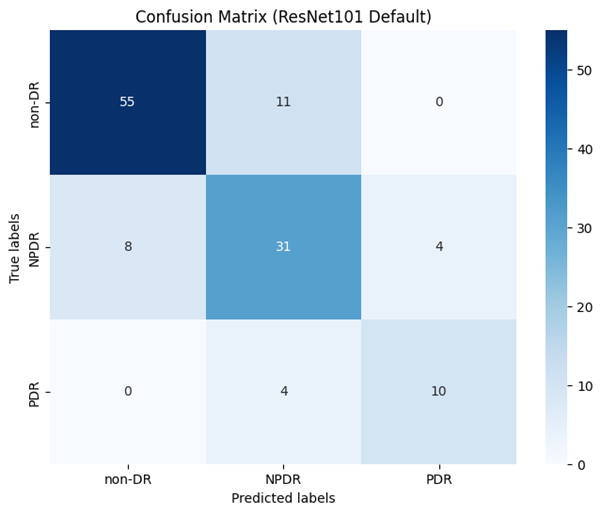
\includegraphics[width=7cm]{gambar/confusionMatrixResnet101_bestTrain.png} }}%
	\qquad
	\subfloat[\centering Best Val acc ResNet-101]{{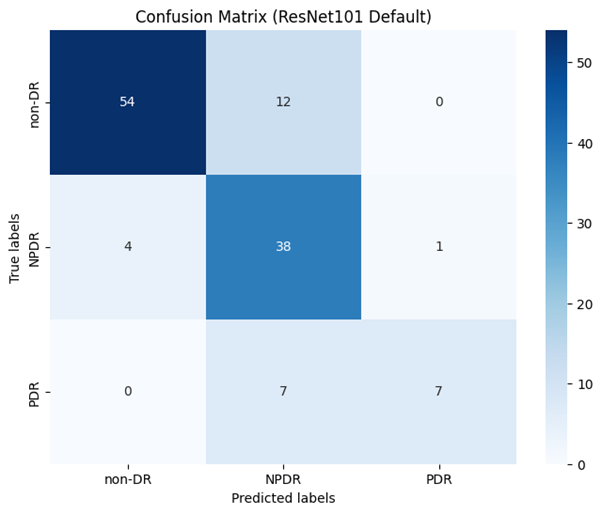
\includegraphics[width=7cm]{gambar/confusionMatrixResnet101_bestVal.png} }}%
	\qquad
	\subfloat[\centering Last Trained ResNet-101]{{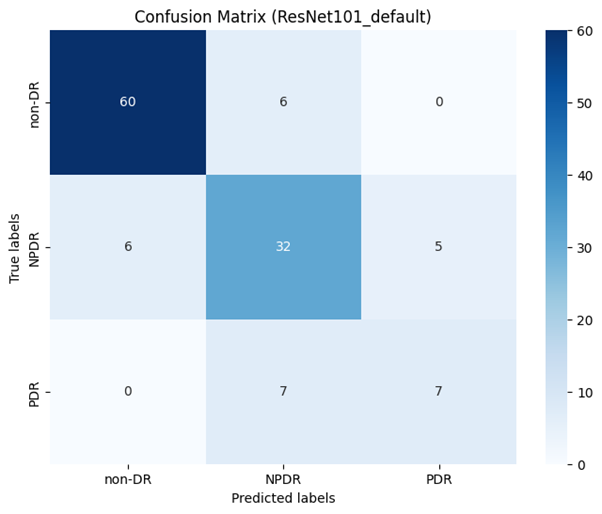
\includegraphics[width=7cm]{gambar/last model/confusionMatrixResnet101.png} }}%
	\caption{Confusion Matrix ResNet-101 yang Tidak Dilakukan Penyesuaian Beban Kelas}
	\label{fig:confRes101}
\end{figure}

\begin{itemize}
	\item Untuk dataset non-DR dapat dilihat bahwa model dapat melakukan prediksi \textbf{60 kasus non-DR} dengan akurat, dan 6 kasus diprediksi salah sebagai NDPR tanpa prediksi untuk PDR.
	
	\item Untuk dataset NPDR dapat dilihat bahwa model dapat melakukan prediksi \textbf{38 kasus NPDR} dengan akurat, 4 kasus diprediksi sebagai non-DR, dan 1 kasus diprediksi sebagai PDR.
	
	\item Untuk dataset PDR dapat dilihat bahwa model dapat melakukan prediksi \textbf{10 kasus PDR} dengan akurat, dan 4 kasus diprediksi sebagai NPDR tanpa prediksi non-DR.
\end{itemize}
\pagebreak

\begin{figure}[hbtp]
	\centering
	\subfloat[\centering Best Train acc ResNet-152]{{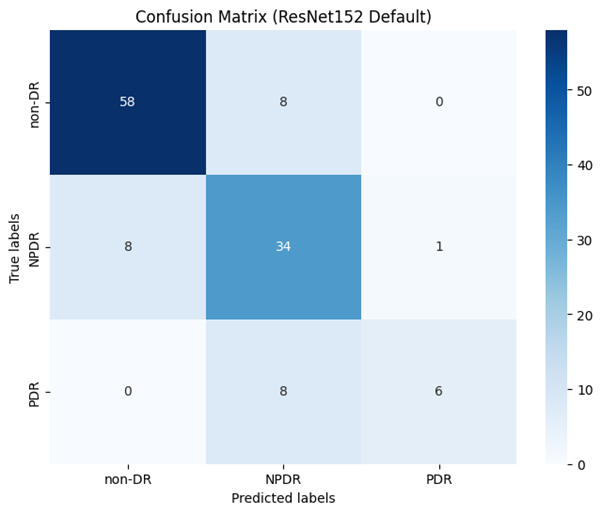
\includegraphics[width=7cm]{gambar/confusionMatrixResnet152_bestTrain.png} }}%
	\qquad
	\subfloat[\centering Best Val acc ResNet-152]{{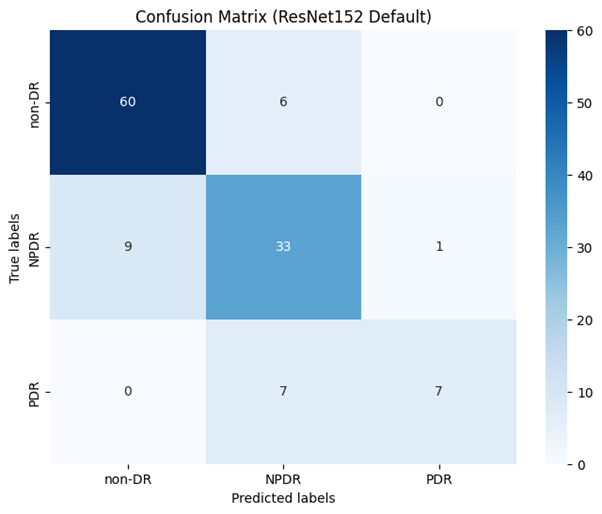
\includegraphics[width=7cm]{gambar/confusionMatrixResnet152_bestVal.png} }}%
	\qquad
	\subfloat[\centering Last Trained ResNet-152]{{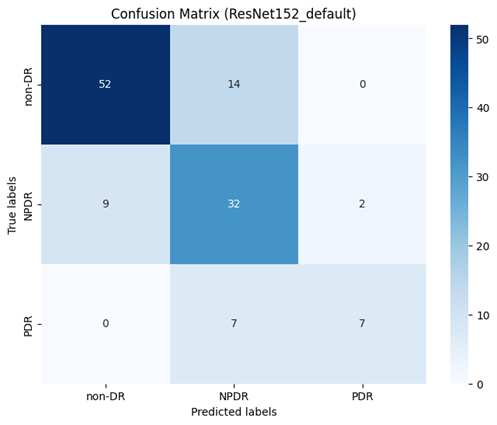
\includegraphics[width=7cm]{gambar/last model/confusionMatrixResnet152.png} }}%
	\caption{Confusion Matrix ResNet-152 yang Tidak Dilakukan Penyesuaian Beban Kelas}
	\label{fig:confRes152}
\end{figure}
\FloatBarrier

\begin{itemize}
	\item Untuk dataset non-DR dapat dilihat bahwa model terbaik adalah model best \emph{validation accuracy}, yang dapat melakukan prediksi \textbf{60 kasus non-DR} dengan akurat, dan 6 kasus diprediksi salah sebagai NDPR tanpa kasus diprediksi sebagai PDR.
	
	\item Untuk dataset NPDR dapat dilihat bahwa model terbaik adalah model \emph{best train accuracy}, yang dapat melakukan prediksi \textbf{34 kasus NPDR} dengan akurat, 8 kasus diprediksi sebagai non-DR, dan 1 kasus diprediksi sebagai PDR.
	
	\item Untuk dataset PDR dapat dilihat bahwa model terbaik adalah model \emph{best validation accuracy} dapat melakukan prediksi \textbf{7 kasus PDR} dengan akurat, 7 kasus diprediksi sebagai NPDR tanpa kasus diprediksi sebagai non-DR.
\end{itemize}
\pagebreak

\subsection{Hasil Pengujian Model dengan Menggunakan Penyesuaian class-weight}
\label{sec:412}
Proses testing untuk mendapatkan nilai QWK dilakukan dengan menggunakan data yang tidak dipergunakan saat training sebelumnya. Namun karena dataset testing tidak memiliki label, untuk metrik \emph{precision, recall}, dan \emph{F1-score} digunakan dataset validasi, yang sebesar 10\% dari dataset training. Model yang digunakan adalah model dengan metrik validasi terbaik, training terbaik, dan model terakhir dari setiap arsitektur.  Hasil pengujian metrik yang telah disebutkan dapat dilihat pada tabel \ref{tb:HasilTrainClassWeight}, tabel \ref{tb:HasilValClassWeight}, dan tabel \ref{tb:HasilLastClassWeight}
\begin{table}[hbtp]
	\begin{center}
		\caption{Hasil best trained model menggunakan Penyesuaian Beban Class}
		\label{tb:HasilTrainClassWeight}
		\begin{tabular}{|c|l|c|l|l|l|c|}
			\hline
			\rowcolor[HTML]{C0C0C0} 
			Arsitektur & \multicolumn{1}{c|}{\cellcolor[HTML]{C0C0C0}class} & acc                      & \multicolumn{1}{c|}{\cellcolor[HTML]{C0C0C0}prec} & \multicolumn{1}{c|}{\cellcolor[HTML]{C0C0C0}rec} & \multicolumn{1}{c|}{\cellcolor[HTML]{C0C0C0}F1} & QWK                                  \\ \hline
			& non-DR                                             &                          & 0,875                                             & \textbf{0,848485}                                & 0,861538                                        &                                      \\ \cline{2-2} \cline{4-6}
			& NPDR                                               &                          & 0,704545                                          & \textbf{0,72093}                                 & \textbf{0,712644}                               &                                      \\ \cline{2-2} \cline{4-6}
			\multirow{-3}{*}{ResNet-18}  & PDR                                                & \multirow{-3}{*}{\textbf{0,7886}} & \textbf{0,666667}                        & 0,714286                                         & 0,689655                                        & \multirow{-3}{*}{\textbf{0.7526956474324895}} \\ \hline
			& non-DR                                             &                          & 0,877193                                          & 0,757576                                         & 0,813008                                        &                                      \\ \cline{2-2} \cline{4-6}
			& NPDR                                               &                          & 0,617021                                          & 0,674419                                         & 0,644444                                        &                                      \\ \cline{2-2} \cline{4-6}
			\multirow{-3}{*}{ResNet-34}  & PDR                                                & \multirow{-3}{*}{0,7236} & 0,526316                                          & 0,714286                                         & 0,606061                                        & \multirow{-3}{*}{0.7344195070936137} \\ \hline
			& non-DR                                             &                          & 0,848485                                          & \textbf{0,848485}                                & 0,848485                                        &                                      \\ \cline{2-2} \cline{4-6}
			& NPDR                                               &                          & 0,634146                                          & 0,604651                                         & 0,619048                                        &                                      \\ \cline{2-2} \cline{4-6}
			\multirow{-3}{*}{ResNet-50}  & PDR                                                & \multirow{-3}{*}{0,7317} & 0,5                                               & 0,571429                                         & 0,533333                                        & \multirow{-3}{*}{0.7416221605070141} \\ \hline
			& non-DR                                             &                          & \textbf{0,916667}                                 & 0,833333                                         & \textbf{0,873016}                               &                                      \\ \cline{2-2} \cline{4-6}
			& NPDR                                               &                          & 0,666667                                          & 0,651163                                         & 0,658824                                        &                                      \\ \cline{2-2} \cline{4-6}
			\multirow{-3}{*}{ResNet-101} & PDR                                                & \multirow{-3}{*}{0,7642} & 0,52381                                           & 0,785714                                         & 0,628571                                        & \multirow{-3}{*}{0.7133252550521831} \\ \hline
			& non-DR                                             &                          & 0,870968                                          & 0,818182                                         & 0,84375                                         &                                      \\ \cline{2-2} \cline{4-6}
			& NPDR                                               &                          & \textbf{0,714286}                                 & 0,697674                                         & 0,705882                                        &                                      \\ \cline{2-2} \cline{4-6}
			\multirow{-3}{*}{ResNet-152} & PDR                                                & \multirow{-3}{*}{0,7805} & 0,631579                                          & \textbf{0,857143}                                & \textbf{0,727273}                               & \multirow{-3}{*}{0.7423939072743689} \\ \hline
		\end{tabular}
	\end{center}
\end{table}

Dari model terakhir yang telah dilatih, didapatkan nilai akurasi terbaik sebesar \textbf{0,7886} dari arsitektur \emph{ResNet-18}.

\begin{itemize}
	
	\item Untuk dataset non-DR didapatkan nilai precision sebesar \textbf{0,916667} dari arsitektur \emph{ResNet-101}, recall \textbf{0,848485} yang didapatkan pada arsitektur \emph{Resnet-18} dan \emph{ResNet-50}, dan F1 sebesar \textbf{0,873016} dari arsitektur \emph{ResNet-101};
	
	\item Untuk dataset NPDR didapatkan nilai precision sebesar \textbf{0,714286} dari arsitektur \emph{ResNet-152}, nilai recall sebesar \textbf{0,72093} dari arsitektur \emph{ResNet-18}, nilai F1 sebesar \textbf{0,712644} dari arsitektur \emph{ResNet-18};
	
	\item Untuk dataset PDR didapatkan nilai precision sebesar \textbf{0,667} dari arsitektur \emph{ResNet-18}, nilai recall sebesar \textbf{0,857143} dari arsitektur \emph{ResNet-152}, nilai F1 sebesar \textbf{0,727273} dari arsitektur \emph{ResNet-152}.
	
\end{itemize}

Dari seluruh arsitektur \emph{ResNet} yang digunakan, nilai QWK tertinggi sebesar \textbf{0.7526956474324895} didapatkan dari arsitektur \emph{ResNet-18}. Untuk hasil dari best validated model dari setiap arsitektur ResNet dapat dilihat pada tabel \ref{tb:HasilValClassWeight}

\pagebreak

\begin{table}[H]
	\begin{center}
		\caption{Hasil best validated model menggunakan Penyesuaian Beban Class}
		\label{tb:HasilValClassWeight}
		\begin{tabular}{|c|l|c|l|l|l|c|}
			\hline
			\rowcolor[HTML]{C0C0C0} 
			Arsitektur & \multicolumn{1}{c|}{\cellcolor[HTML]{C0C0C0}class} & acc                      & prec     & rec      & F1       & QWK                                  \\ \hline
			& non-DR                                             &                          & 0,869565 & 0,909091 & 0,888889 &                                      \\ \cline{2-2} \cline{4-6}
			& NPDR                                               &                          & 0,717391 & \textbf{0,767442} & 0,741573 &                             \\ \cline{2-2} \cline{4-6}
			\multirow{-3}{*}{ResNet-18}  & PDR                                                & \multirow{-3}{*}{\textbf{0,813}}  & \textbf{0,875}    & 0,5      & 0,636364 & \multirow{-3}{*}{0.6266311390141076} \\ \hline
			& non-DR                                             &                          & 0,777778 & \textbf{0,954545} & 0,857143 &                             \\ \cline{2-2} \cline{4-6}
			& NPDR                                               &                          & \textbf{0,88}     & 0,511628 & 0,647059 &                              \\ \cline{2-2} \cline{4-6}
			\multirow{-3}{*}{ResNet-34}  & PDR                                                & \multirow{-3}{*}{0,7886} & 0,705882 & \textbf{0,857143} & 0,774194 & \multirow{-3}{*}{0.6915275416648504} \\ \hline
			& non-DR                                             &                          & 0,84058  & 0,878788 & 0,859259 &                                      \\ \cline{2-2} \cline{4-6}
			& NPDR                                               &                          & 0,690476 & 0,674419 & 0,682353 &                                      \\ \cline{2-2} \cline{4-6}
			\multirow{-3}{*}{ResNet-50}  & PDR                                                & \multirow{-3}{*}{0,7805} & 0,75     & 0,642857 & 0,692308 & \multirow{-3}{*}{\textbf{0.7084479219119185}} \\ \hline
			& non-DR                                             &                          & \textbf{0,907692} & 0,893939 & \textbf{0,900763} &                    \\ \cline{2-2} \cline{4-6}
			& NPDR                                               &                          & 0,72973  & 0,627907 & 0,675    &                                      \\ \cline{2-2} \cline{4-6}
			\multirow{-3}{*}{ResNet-101} & PDR                                                & \multirow{-3}{*}{0,7886} & 0,52381  & 0,785714 & 0,628571 & \multirow{-3}{*}{0.7076588090504592} \\ \hline
			& non-DR                                             &                          & 0,870968 & 0,818182 & 0,84375  &                                      \\ \cline{2-2} \cline{4-6}
			& NPDR                                               &                          & 0,733333 & \textbf{0,767442} & \textbf{0,75}     &                    \\ \cline{2-2} \cline{4-6}
			\multirow{-3}{*}{ResNet-152} & PDR                                                & \multirow{-3}{*}{0,8049} & 0,75     & \textbf{0,857143} & \textbf{0,8}      & \multirow{-3}{*}{0.7052973650209466} \\ \hline
		\end{tabular}
	\end{center}
\end{table}

Dari model terakhir yang telah dilatih, didapatkan nilai akurasi terbaik sebesar \textbf{0,813} dari arsitektur \emph{ResNet-18}.

\begin{itemize}
	
	\item Untuk dataset non-DR didapatkan nilai precision sebesar \textbf{0,907692} dari arsitektur \emph{ResNet-101}, recall \textbf{0,954545} dari arsitektur \emph{ResNet-34}, dan F1 sebesar \textbf{0,900763} dari arsitektur \emph{ResNet-101};
	
	\item Untuk dataset NPDR didapatkan nilai precision sebesar \textbf{0,88} dari arsitektur \emph{ResNet-34}, nilai recall sebesar \textbf{0,767442} dari arsitektur \emph{ResNet-18} dan \textbf{0,767442}, nilai F1 sebesar \textbf{0,75} dari arsitektur \emph{ResNet-152};
	
	\item Untuk dataset PDR didapatkan nilai precision sebesar \textbf{0,875} dari arsitektur \emph{ResNet-18}, nilai recall sebesar \textbf{0,857143} dari arsitektur \emph{ResNet-34} dan arsitektur \emph{ResNet-152}, nilai F1 sebesar \textbf{0,8} dari arsitektur \emph{ResNet-152}.
	
\end{itemize}

Dari seluruh arsitektur \emph{ResNet} yang digunakan, nilai QWK tertinggi sebesar \textbf{0.7084479219119185} didapatkan dari arsitektur \emph{ResNet-50}. Untuk hasil dari model epoch terakhir dari setiap arsitektur ResNet dapat dilihat pada tabel \ref{tb:HasilLastClassWeight}

\pagebreak

\begin{table}[hbtp]
	\begin{center}
		\caption{Hasil Last Trained Model Menggunakan Penyesuaian Beban Class}
		\label{tb:HasilLastClassWeight}
		\begin{tabular}{|c|l|c|l|l|l|c|}
			\hline
			\rowcolor[HTML]{C0C0C0} 
			Arsitektur & \multicolumn{1}{c|}{\cellcolor[HTML]{C0C0C0}class} & acc                      & \multicolumn{1}{c|}{\cellcolor[HTML]{C0C0C0}prec} & \multicolumn{1}{c|}{\cellcolor[HTML]{C0C0C0}rec} & \multicolumn{1}{c|}{\cellcolor[HTML]{C0C0C0}F1} & QWK                                  \\ \hline
			& non-DR                                             &                          & 0,852941                                          & 0,878788                                         & 0,865672                                        &                                      \\ \cline{2-2} \cline{4-6}
			& NPDR                                               &                          & 0,710526                                          & 0,627907                                         & 0,666667                                        &                                      \\ \cline{2-2} \cline{4-6}
			\multirow{-3}{*}{ResNet-18}  & PDR                                                & \multirow{-3}{*}{\textbf{0,7724}} & 0,588235                                 & 0,714286                                         & 0,645161                                        & \multirow{-3}{*}{0.714979444673576}  \\ \hline
			& non-DR                                             &                          & 0,857143                                          & 0,818182                                         & 0,837209                                        &                                      \\ \cline{2-2} \cline{4-6}
			& NPDR                                               &                          & 0,652174                                          & 0,697674                                         & 0,674157                                        &                                      \\ \cline{2-2} \cline{4-6}
			\multirow{-3}{*}{ResNet-34}  & PDR                                                & \multirow{-3}{*}{0,748}  & 0,571429                                          & 0,571429                                         & 0,571429                                        & \multirow{-3}{*}{0.7137225555570403} \\ \hline
			& non-DR                                             &                          & 0,822581                                          & 0,772727                                         & 0,796875                                        &                                      \\ \cline{2-2} \cline{4-6}
			& NPDR                                               &                          & 0,608696                                          & 0,651163                                         & 0,629213                                        &                                      \\ \cline{2-2} \cline{4-6}
			\multirow{-3}{*}{ResNet-50}  & PDR                                                & \multirow{-3}{*}{0,7236} & 0,666667                                          & 0,714286                                         & 0,689655                                        & \multirow{-3}{*}{0.7006591702210159} \\ \hline
			& non-DR                                             &                          & 0,901639                                          & 0,833333                                         & 0,866142                                        &                                      \\ \cline{2-2} \cline{4-6}
			& NPDR                                               &                          & 0,666667                                          & 0,697674                                         & 0,681818                                        &                                      \\ \cline{2-2} \cline{4-6}
			\multirow{-3}{*}{ResNet-101} & PDR                                                & \multirow{-3}{*}{\textbf{0,7724}} & 0,588235                                 & 0,714286                                         & 0,645161                                        & \multirow{-3}{*}{\textbf{0.7422994855414904}} \\ \hline
			& non-DR                                             &                          & 0,892857                                          & 0,757576                                         & 0,819672                                        &                                      \\ \cline{2-2} \cline{4-6}
			& NPDR                                               &                          & 0,604167                                          & 0,674419                                         & 0,637363                                        &                                      \\ \cline{2-2} \cline{4-6}
			\multirow{-3}{*}{ResNet-152} & PDR                                                & \multirow{-3}{*}{0,7154} & 0,473684                                          & 0,642857                                         & 0,545455                                        & \multirow{-3}{*}{0.727319861566579}  \\ \hline
		\end{tabular}
	\end{center}
\end{table}

Dari model terakhir yang telah dilatih, didapatkan nilai akurasi terbaik sebesar \textbf{0,7724} dari arsitektur \emph{ResNet-18} dan \emph{ResNet-101}.

\begin{itemize}
	
	\item Untuk dataset non-DR didapatkan nilai precision sebesar \textbf{0,907692} dari arsitektur \emph{ResNet-101}, recall \textbf{0,954545} dari arsitektur \emph{ResNet-34}, dan F1 sebesar \textbf{0,900763} dari arsitektur \emph{ResNet-101};
	
	\item Untuk dataset NPDR didapatkan nilai precision sebesar \textbf{0,88} dari arsitektur \emph{ResNet-34}, nilai recall sebesar \textbf{0,767442} dari arsitektur \emph{ResNet-18} dan \textbf{0,767442}, nilai F1 sebesar \textbf{0,75} dari arsitektur \emph{ResNet-152};
	
	\item Untuk dataset PDR didapatkan nilai precision sebesar \textbf{0,875} dari arsitektur \emph{ResNet-18}, nilai recall sebesar \textbf{0,857143} dari arsitektur \emph{ResNet-34} dan arsitektur \emph{ResNet-152}, nilai F1 sebesar \textbf{0,8} dari arsitektur \emph{ResNet-152}.
	
\end{itemize}

Dari seluruh arsitektur \emph{ResNet} yang digunakan, nilai QWK tertinggi sebesar \textbf{0.7422994855414904} didapatkan dari arsitektur \emph{ResNet-101}.

Grafik dari \emph{training loss}, \emph{training accuracy}, dan \emph{validation accuracy} pada setiap arsitektur tanpa menggunakan penyesuaian \emph{class weight} dapat dilihat dengan lebih jelas pada Gambar \ref{Fig:GraphTrainingDefPt2} Nilai loss cukup tinggi pada permulaan dikarenakan ukuran \emph{batch} yang cukup kecil, sehingga jumlah training sample yang digunakan dalam satu batch untuk satu iterasi juga kecil. Namun, setelah epoch tertentu, model akan menjaga nilai loss-nya tetap stabil pada nilai yang relatif rendah.
\pagebreak

\begin{figure}[hbtp]
	\centering
	\subfloat[\centering Training Loss dan akurasi ResNet-18]{{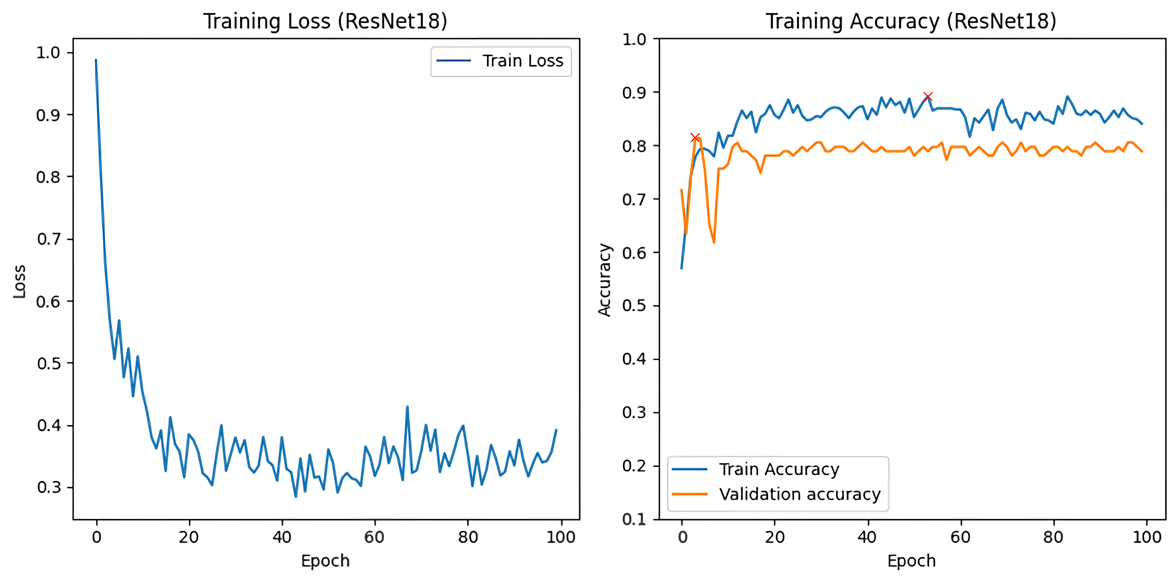
\includegraphics[height=7cm]{gambar/TrainingGraphResNet18class-weighted.png}}}
	\qquad
	\subfloat[\centering Training Loss dan akurasi ResNet-34]{{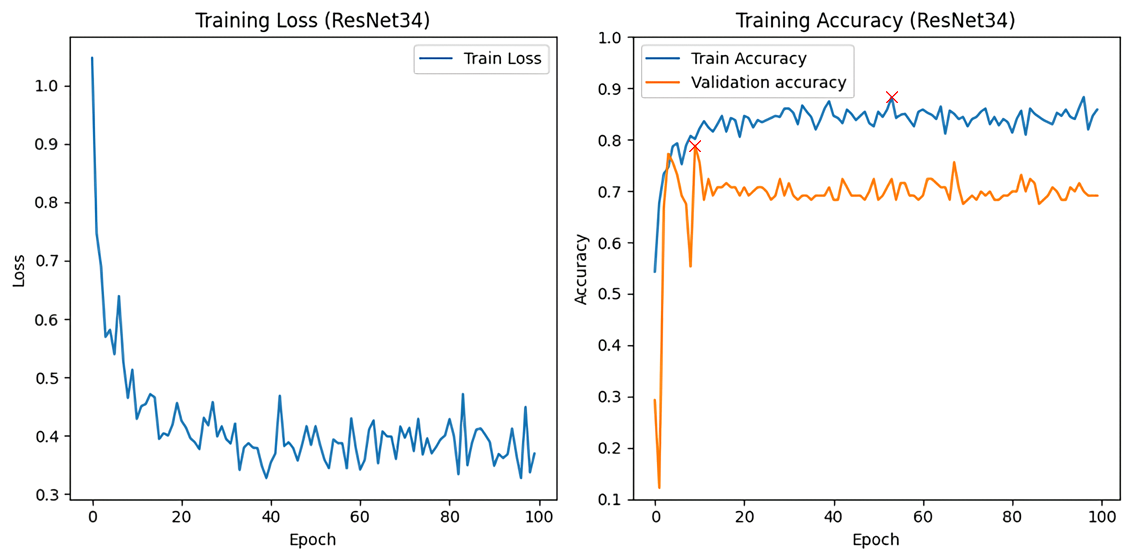
\includegraphics[height=7cm]{gambar/TrainingGraphResNet34class-weighted.png}}}
	\caption{Grafik Training Loss dan akurasi ResNet-18 dan ResNet-34 dengan Penyesuaian Beban pada \emph{Class}}
	\label{fig:graphTrainingWeightedPt1}
\end{figure}

Dari grafik Training Loss \emph{ResNet-18} dapat dilihat bahwa nilai loss mulai dari \textbf{1.0} dan dengan cepat menjadi stabil mendekati epoch ke-\textbf{20} dengan nilai menjadi fluktuatif di antara \textbf{0.3 dan 0.45}.

Dari grafik Training Accuracy \emph{ResNet-18} dapat dilihat bahwa akurasi training mulai dari nilai \textbf{0.6} dan dengan cepat menjadi stabil mendekati epoch ke-\textbf{10} dimana nilai berada di antara \textbf{0.8 dan 0.9} 

Dari grafik Training Accuracy \emph{ResNet-18} dapat dilihat bahwa akurasi validasi mulai dari nilai \textbf{0.7} dan bersifat fluktuatif hingga epoch ke-\textbf{20} dimana nilai menjadi stabil di antara \textbf{0.7 dan 0.8}.

Kemudian Dari grafik Training Loss \emph{ResNet-34} dapat dilihat bahwa nilai loss mulai dari \textbf{1.0} dan dengan cepat menjadi stabil mendekati epoch ke-\textbf{20} dengan nilai menjadi fluktuatif di antara \textbf{0.3 dan 0.5}.

Dari grafik Training Accuracy \emph{ResNet-34} dapat dilihat bahwa akurasi training mulai dari nilai \textbf{0.55} dan dengan cepat menjadi stabil mendekati epoch ke-\textbf{10} dimana nilai berada di antara \textbf{0.8 dan 0.9} 

Dari grafik Training Accuracy \emph{ResNet-34} dapat dilihat bahwa akurasi validasi mulai dari nilai \textbf{0.3}, kemudian turun mendekati nilai \textbf{0.1} sebelum kemudian naik kembali dan bersifat fluktuatif hingga epoch ke-\textbf{20} dimana nilai menjadi stabil di antara \textbf{0.7 dan 0.8}.

\begin{figure}[H]
	\centering
	\subfloat[\centering Training Loss dan akurasi ResNet-50]{{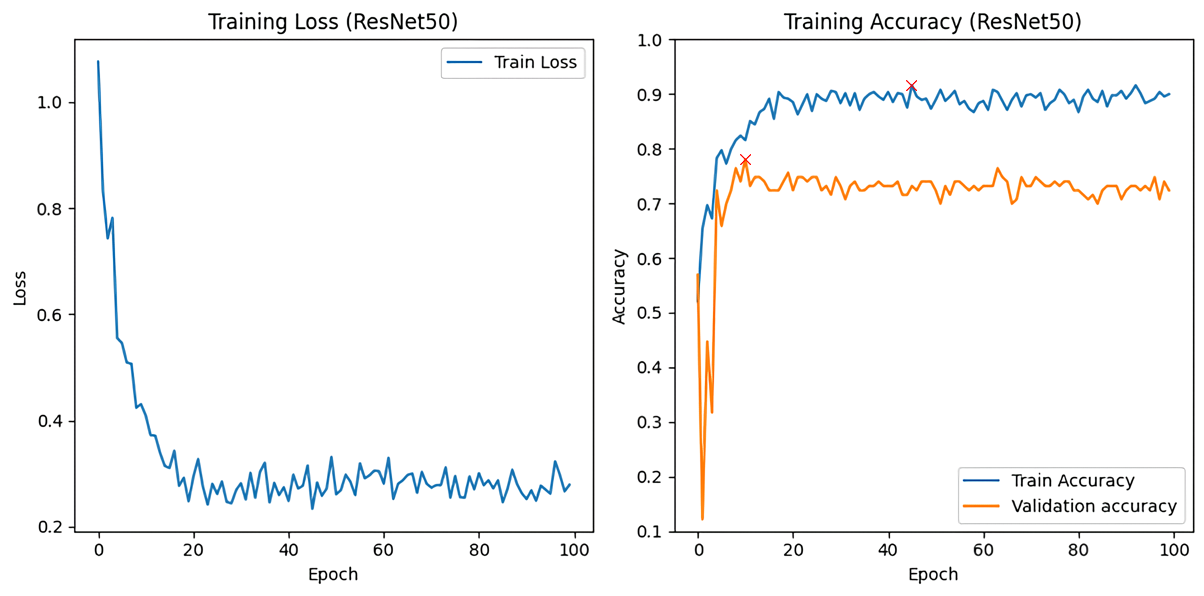
\includegraphics[height=7cm]{gambar/TrainingGraphResNet50class-weighted.png}}}
	\qquad
	\subfloat[\centering Training Loss dan akurasi ResNet-101]{{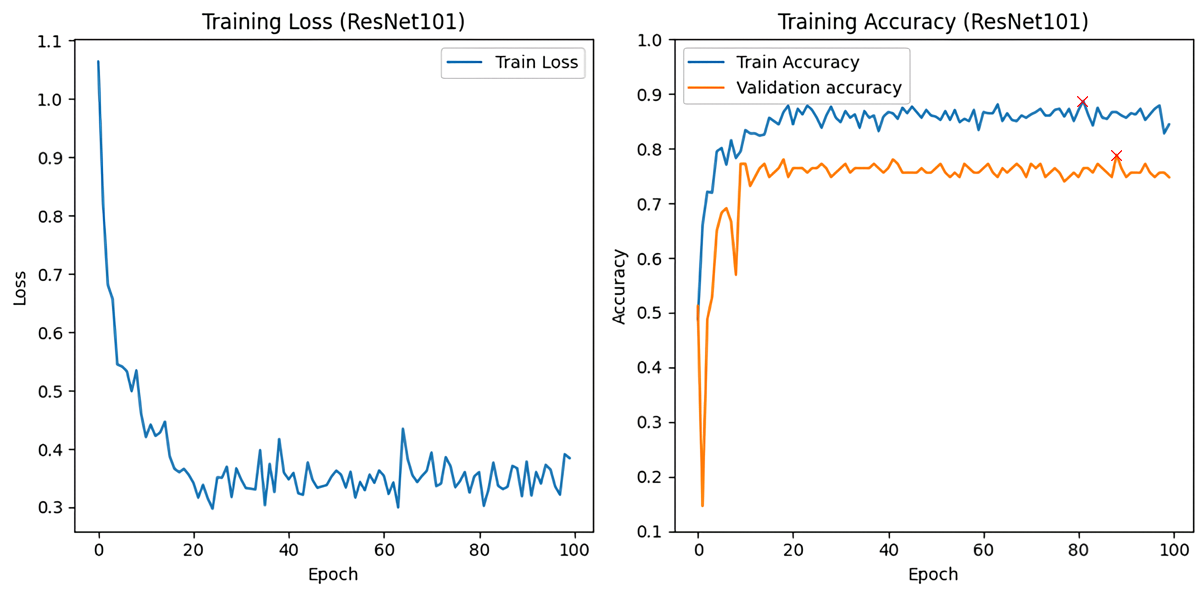
\includegraphics[height=7cm]{gambar/TrainingGraphResNet101class-weighted.png}}}
	\caption{Grafik Training Loss dan akurasi ResNet-50, 101 dengan Penyesuaian Beban pada \emph{Class}}
	\label{fig:graphTrainingWeightedPt2}
\end{figure}

Dari grafik Training Loss \emph{ResNet-50} dapat dilihat bahwa nilai loss mulai dari \textbf{1.05} dan dengan cepat menjadi stabil mendekati epoch ke-\textbf{20} dengan nilai menjadi fluktuatif di antara \textbf{0.3 dan 0.4}.

Dari grafik Training Accuracy \emph{ResNet-50} dapat dilihat bahwa akurasi training mulai dari nilai mendekati \textbf{0.6} dan dengan cepat menjadi stabil mendekati epoch ke-\textbf{10} dimana nilai berada di antara \textbf{0.8 dan 0.9} 

Dari grafik Training Accuracy \emph{ResNet-50} dapat dilihat bahwa akurasi validasi mulai dari nilai \textbf{0.6} kemudian turun mendekati \textbf{0.1} sebelum akhirnya naik kembali, dan bersifat fluktuatif hingga epoch ke-\textbf{10} dimana nilai menjadi stabil di antara \textbf{0.7 dan 0.8}.

Kemudian Dari grafik Training Loss \emph{ResNet-101} dapat dilihat bahwa nilai loss mulai dari mendekati \textbf{1.1} dan dengan cepat menjadi stabil mendekati epoch ke-\textbf{20} dengan nilai menjadi fluktuatif di antara \textbf{0.3 dan 0.45}.

Dari grafik Training Accuracy \emph{ResNet-101} dapat dilihat bahwa akurasi training mulai dari nilai \textbf{0.6} dan dengan cepat menjadi stabil mendekati epoch ke-\textbf{10} dimana nilai berada di antara \textbf{0.8 dan 0.9} 

Dari grafik Training Accuracy \emph{ResNet-101} dapat dilihat bahwa akurasi validasi mulai dari nilai \textbf{0.5} kemudian turun mendekati \textbf{0.1} sebelum akhirnya naik kembali dan bersifat fluktuatif hingga sebelum epoch ke-\textbf{20} dimana nilai menjadi stabil di antara \textbf{0.7 dan 0.8}.

\begin{figure}[H]
	\centering
	\subfloat[\centering Training Loss dan akurasi ResNet-152]{{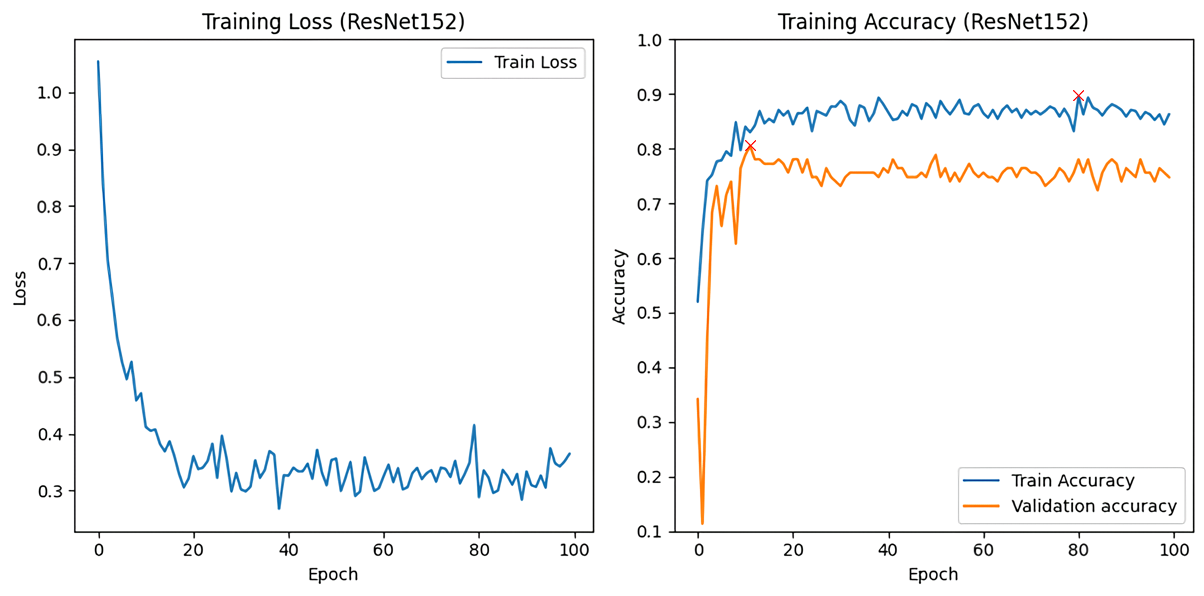
\includegraphics[height=7cm]{gambar/TrainingGraphResNet152class-weighted.png}}}
	\caption{Grafik Training Loss dan akurasi ResNet-152 dengan Penyesuaian Beban pada \emph{Class}}
	\label{fig:graphTrainingWeightedPt3}
\end{figure}
Dari grafik Training Loss \emph{ResNet-152} dapat dilihat bahwa nilai loss mulai dari \textbf{\>1.0} dan dengan cepat menjadi stabil mendekati epoch ke-\textbf{20} dengan nilai menjadi fluktuatif di antara \textbf{0.3 dan 0.45}.

Dari grafik Training Accuracy \emph{ResNet-152} dapat dilihat bahwa akurasi training mulai dari nilai \textbf{\>0.5} dan dengan cepat menjadi stabil mendekati epoch ke-\textbf{10} dimana nilai berada di antara \textbf{0.8 dan 0.9} 

Dari grafik Training Accuracy \emph{ResNet-152} dapat dilihat bahwa akurasi validasi mulai dari nilai antara \textbf{0.3} dan \textbf{0.4} kemudian turun mendekati \textbf{0.1} sebelum akhirnya naik dan bersifat fluktuatif hingga epoch ke-\textbf{20}. Dimana nilai menjadi stabil di antara \textbf{0.7 dan 0.8}.

Untuk \emph{confusion matrix} dari setiap arsitektur dapat dilihat pada Gambar \ref{fig:confRes18Class}, Gambar \ref{fig:confRes34Class}, Gambar \ref{fig:confRes50Class}, Gambar \ref{fig:confRes101Class}, dan Gambar \ref{fig:confRes152Class}. Masing - masing gambar terdiri dari tiga \emph{confusion matrix}, yang merupakan hasil dari model terbaik pada akurasi \emph{training}, model terbaik pada akurasi validasi, dan model terakhir dari 100 \emph{epoch} pada arsitektur tersebut.

\begin{figure}[hbtp]
	\centering
	\subfloat[\centering Best Train acc ResNet-18]{{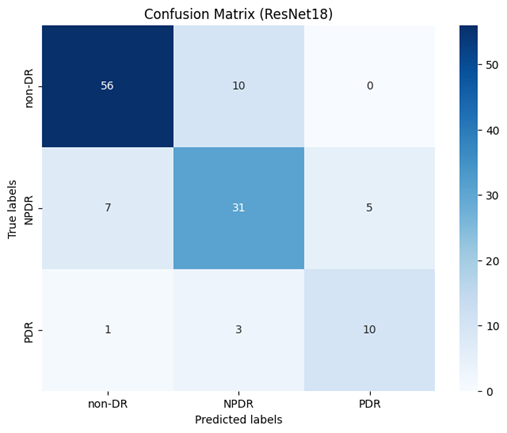
\includegraphics[width=7cm]{gambar/confusionMatrixResnet18class-weighted_bestTrain.png} }}%
	\qquad
	\subfloat[\centering Best Val acc ResNet-18]{{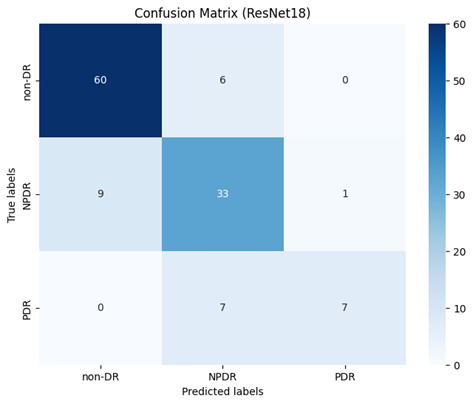
\includegraphics[width=7cm]{gambar/confusionMatrixResnet18class-weighted_bestVal.png} }}%
	\qquad
	\subfloat[\centering Last Trained ResNet-18]{{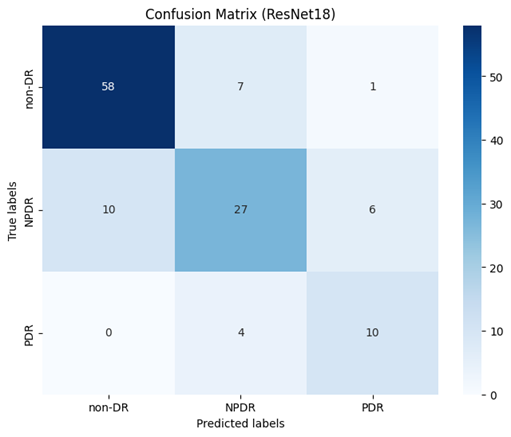
\includegraphics[width=7cm]{gambar/last model/confusionMatrixResnet18class-weighted.png} }}%
	\caption{Confusion Matrix ResNet-18 yang Telah dilakukan Penyesuaian Beban Kelas}
	\label{fig:confRes18Class}
\end{figure}

\begin{itemize}
	\item Untuk dataset non-DR dapat dilihat bahwa model terbaik adalah model \emph{best validation accuracy}, yang dapat melakukan prediksi \textbf{60 kasus non-DR} dengan akurat, dan 6 kasus diprediksi salah sebagai NDPR tanpa prediksi untuk PDR.
	
	\item Untuk dataset NPDR dapat dilihat bahwa model terbaik adalah model \emph{best validation accuracy}, yang dapat melakukan prediksi \textbf{33 kasus NPDR} dengan akurat, 9 kasus diprediksi sebagai non-DR, dan 1 kasus diprediksi sebagai PDR.
	
	\item Untuk dataset PDR dapat dilihat bahwa model terbaik dapat melakukan prediksi \textbf{10 kasus PDR} dengan akurat. Pada model \emph{best train}, 3 kasus diprediksi sebagai NPDR, dan 1 kasus diprediksi sebagai non-DR. Pada model \emph{last trained}, 4 kasus diprediksi sebagai NPDR tanpa prediksi non-DR.
\end{itemize}
\pagebreak

\begin{figure}
	\centering
	\subfloat[\centering Best Train acc ResNet-34]{{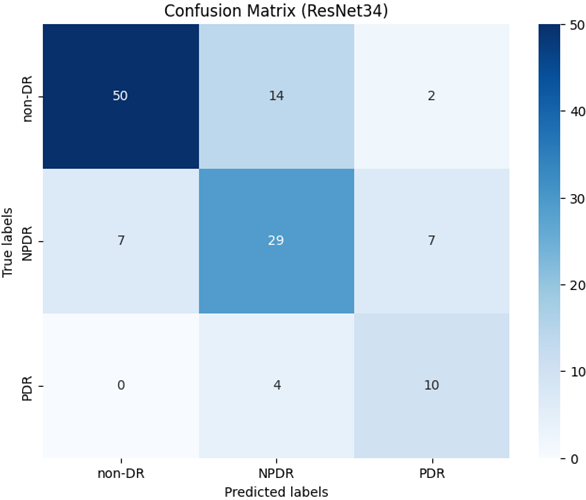
\includegraphics[width=7cm]{gambar/confusionMatrixResnet34class-weighted_bestTrain.png} }}%
	\qquad
	\subfloat[\centering Best Val acc ResNet-34]{{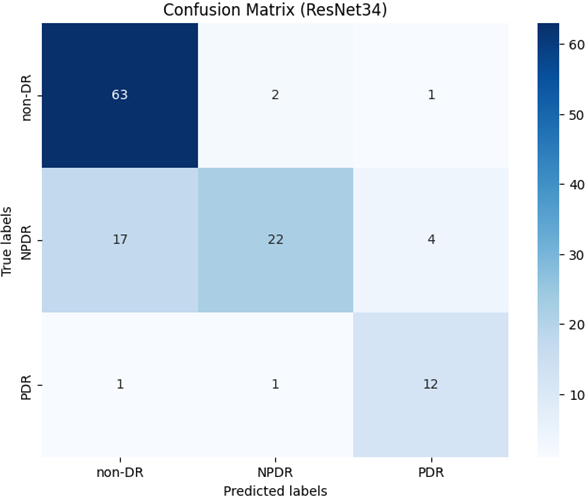
\includegraphics[width=7cm]{gambar/confusionMatrixResnet34class-weighted_bestVal.png} }}%
	\qquad
	\subfloat[\centering Last Trained ResNet-34]{{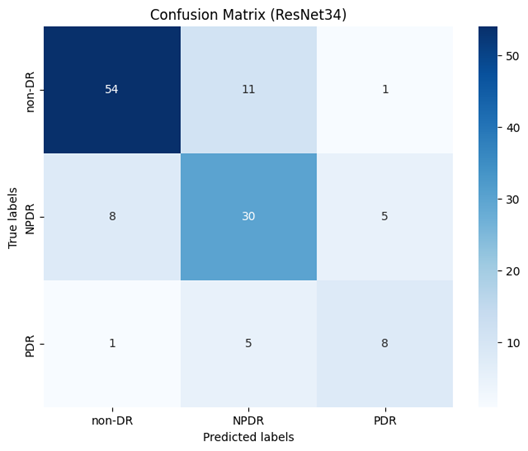
\includegraphics[width=7cm]{gambar/last model/confusionMatrixResnet34class-weighted.png} }}
	\caption{Confusion Matrix ResNet-34 yang Telah dilakukan Penyesuaian Beban Kelas}
	\label{fig:confRes34Class}
\end{figure}

\begin{itemize}
	\item Untuk dataset non-DR dapat dilihat bahwa model terbaik adalah model \emph{best validation accuracy}, yang dapat melakukan prediksi \textbf{63 kasus non-DR} dengan akurat, 2 kasus diprediksi salah sebagai NDPR, dan 1 kasus dirediksi sebagai PDR.
	\item Untuk dataset NPDR dapat dilihat bahwa model terbaik adalah model \emph{last trained}, yang dapat melakukan prediksi \textbf{30 kasus NPDR} dengan akurat, 8 kasus diprediksi sebagai non-DR, dan 5 kasus diprediksi sebagai PDR.
	\item Untuk dataset PDR dapat dilihat bahwa model terbaik adalah model \emph{best validation accuracy}, yang dapat melakukan prediksi \textbf{12 kasus PDR} dengan akurat, 1 kasus diprediksi sebagai NPDR, dan 1 kasus diprediksi sebagai non-DR.
\end{itemize}
\pagebreak

\begin{figure}[hbtp]
	\centering
	\subfloat[\centering Best Train acc ResNet-50]{{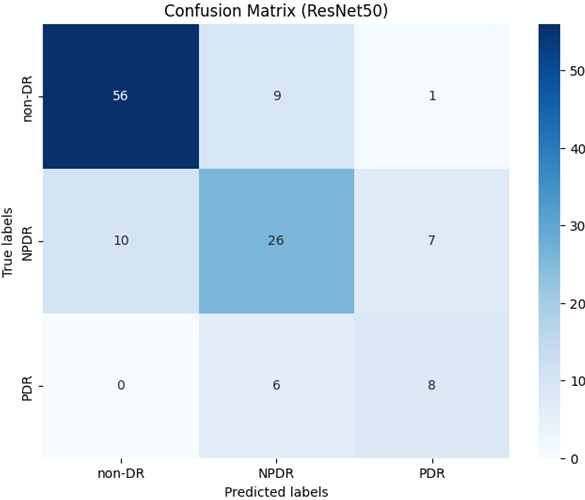
\includegraphics[width=7cm]{gambar/confusionMatrixResnet50class-weighted_bestTrain.png} }}%
	\qquad
	\subfloat[\centering Best Val acc ResNet-50]{{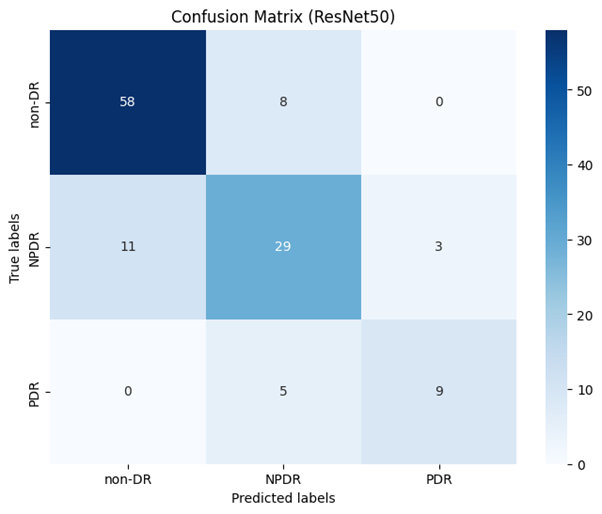
\includegraphics[width=7cm]{gambar/confusionMatrixResnet50class-weighted_bestVal.png} }}%
	\qquad
	\subfloat[\centering Last Trained ResNet-50]{{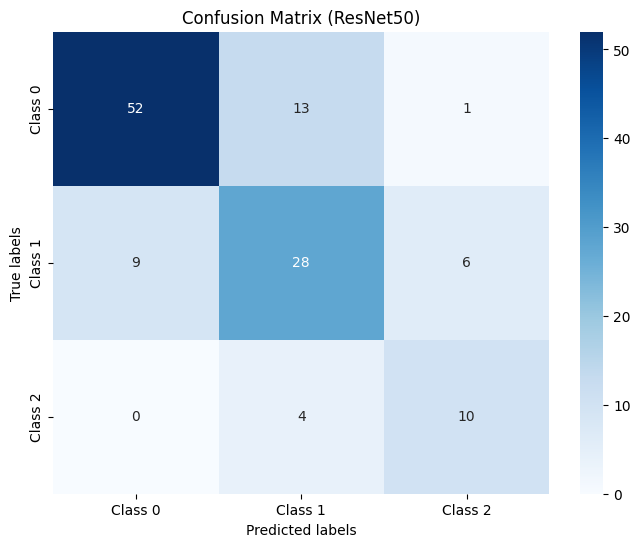
\includegraphics[width=7cm]{gambar/last model/confusionMatrixResnet50class-weighted.png} }}
	\caption{Confusion Matrix ResNet-50 yang Telah dilakukan Penyesuaian Beban Kelas}
	\label{fig:confRes50Class}
\end{figure}

\begin{itemize}
	\item Untuk dataset non-DR dapat dilihat bahwa model terbaik adalah model \emph{best validation accuracy}, yang dapat melakukan prediksi \textbf{58 kasus non-DR} dengan akurat, dan 8 kasus diprediksi salah sebagai NDPR tanpa prediksi untuk PDR.
	
	\item Untuk dataset NPDR dapat dilihat bahwa model terbaik adalah model \emph{best validation accuracy}, yang dapat melakukan prediksi \textbf{29 kasus NPDR} dengan akurat, 11 kasus diprediksi sebagai non-DR, dan 3 kasus diprediksi sebagai PDR.
	
	\item Untuk dataset PDR dapat dilihat bahwa model terbaik adalah model \emph{last trained}, yang dapat melakukan prediksi \textbf{10 kasus PDR} dengan akurat, dan 4 kasus diprediksi sebagai NPDR tanpa prediksi non-DR.
\end{itemize}
\pagebreak

\begin{figure}[hbtp]
	\centering
	\subfloat[\centering Best Train acc ResNet-101]{{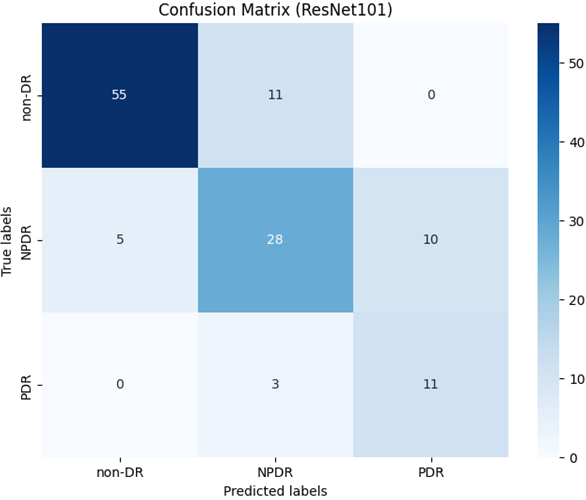
\includegraphics[width=7cm]{gambar/confusionMatrixResnet101class-weighted_bestTrain.png} }}%
	\qquad
	\subfloat[\centering Best Val acc ResNet-101]{{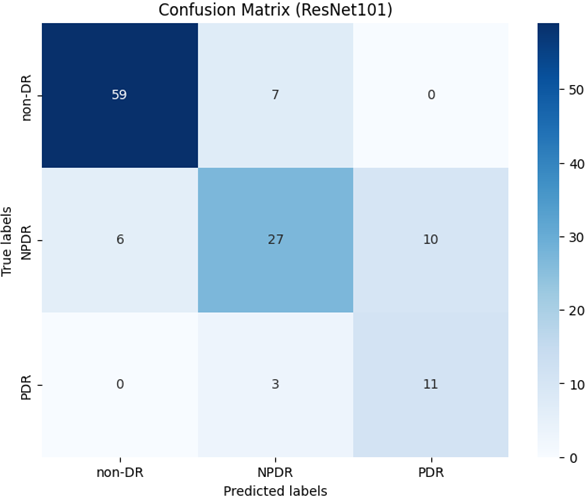
\includegraphics[width=7cm]{gambar/confusionMatrixResnet101class-weighted_bestVal.png} }}%
	\qquad
	\subfloat[\centering Last Trained ResNet-101]{{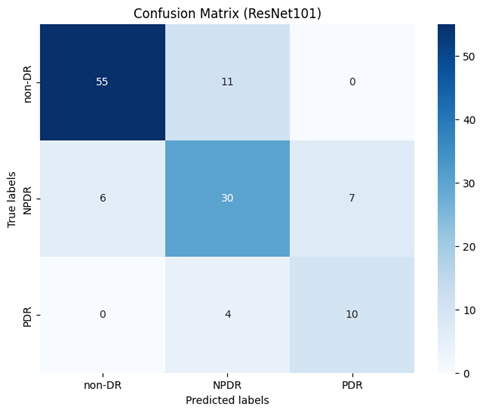
\includegraphics[width=7cm]{gambar/last model/confusionMatrixResnet101class-weighted.png} }}
	\caption{Confusion Matrix ResNet-101 yang Telah dilakukan Penyesuaian Beban Kelas}
	\label{fig:confRes101Class}
\end{figure}

\begin{itemize}
	\item Untuk dataset non-DR dapat dilihat bahwa model terbaik adalah model \emph{best validation accuracy}, yang dapat melakukan prediksi \textbf{59 kasus non-DR} dengan akurat, dan 7 kasus diprediksi salah sebagai NDPR. Tidak ada kasus yang diprediksi sebagai PDR.
	
	\item Untuk dataset NPDR dapat dilihat bahwa model terbaik adalah model \emph{last trained}, yang dapat melakukan prediksi \textbf{30 kasus NPDR} dengan akurat, 6 kasus diprediksi sebagai non-DR, dan 7 kasus diprediksi sebagai PDR.
	
	\item Untuk dataset PDR dapat dilihat bahwa model terbaik adalah model \emph{best train} dan \emph{best validation accuracy}, yang dapat melakukan prediksi \textbf{11 kasus PDR} dengan akurat, 3 kasus diprediksi sebagai NPDR. Tidak ada kasus yang diprediksi sebagai non-DR.
\end{itemize}
\pagebreak

\begin{figure}[hbtp]
	\centering
	\subfloat[\centering Best Train acc ResNet-152]{{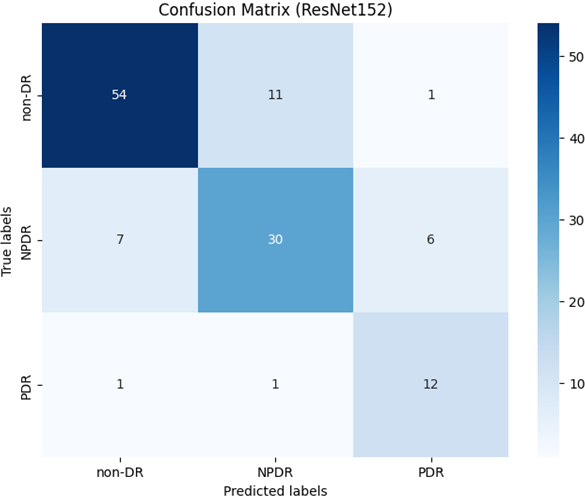
\includegraphics[width=7cm]{gambar/confusionMatrixResnet152class-weighted_bestTrain.png} }}%
	\qquad
	\subfloat[\centering Best Val acc ResNet-152]{{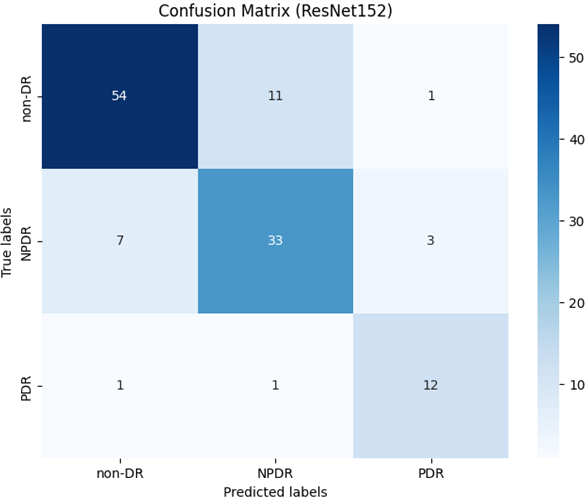
\includegraphics[width=7cm]{gambar/confusionMatrixResnet152class-weighted_bestVal.png} }}%
	\qquad
	\subfloat[\centering Last Trained ResNet-152]{{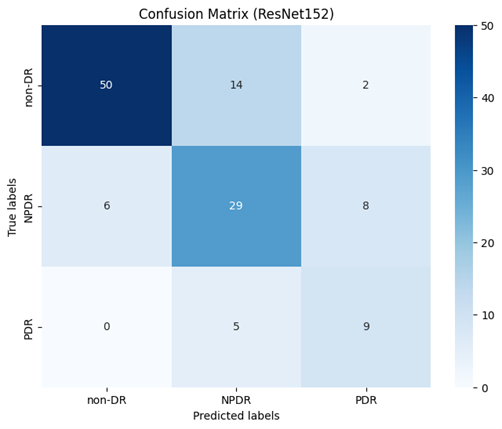
\includegraphics[width=7cm]{gambar/last model/confusionMatrixResnet152class-weighted.png} }}
	\caption{Confusion Matrix ResNet-152 yang Telah dilakukan Penyesuaian Beban Kelas}
	\label{fig:confRes152Class}
\end{figure}

\begin{itemize}
	\item Untuk dataset non-DR dapat dilihat bahwa model terbaik adalah model \emph{best train} dan \emph{best validation accuracy}, yang dapat melakukan prediksi \textbf{54 kasus non-DR} dengan akurat, dan 11 kasus diprediksi salah sebagai NDPR dan 1 kasus diprediksi sebagai PDR.
	
	\item Untuk dataset NPDR dapat dilihat bahwa model terbaik adalah model \emph{best validation accuracy}, yang dapat melakukan prediksi \textbf{33 kasus NPDR} dengan akurat, 7 kasus diprediksi sebagai non-DR, dan 3 kasus diprediksi sebagai PDR.
	
	\item Untuk dataset PDR dapat dilihat bahwa model terbaik adalah model \emph{best validation accuracy}, yang dapat melakukan prediksi \textbf{12 kasus PDR} dengan akurat, 1 kasus diprediksi sebagai NPDR, dan 1 kasus diprediksi sebagai non-DR.
\end{itemize}

\section{Analisis Hasil dan Evaluasi}
\label{sec:42}

Pengujian dilakukan dengan menggunakan model yang memiliki metrik akurasi tertinggi dalam setiap trainingnya. Terdapat dua skenario pengujian yang dilakukan dalam penelitian ini. Pertama, perbandingan untuk setiap arstitektur model yang digunakan tanpa dilakukan penyesuaian pada class-weight. Kedua, perbandingan untuk setiap arstitektur model yang digunakan dengan penerapan class-weight. Hasil perbandingan tersebut akan dilampirkan pada tabel dan nantinya akan dianalisa pada Tabel \ref{tb:PerbandinganHasilBestTrain}, Tabel \ref{tb:PerbandinganHasilBestVal}, dan Tabel \ref{tb:PerbandinganHasilLastTrained}.

\begin{table}[hbtp]
	\begin{center}
	\caption{Perbandingan Nilai Akurasi, Recall pada class PDR. dan QWK dari setiap \emph{Best Trained Model} dengan Pembebanan pada \emph{Class} dan tanpa Pembebanan pada \emph{Class}}
	\label{tb:PerbandinganHasilBestTrain}
	\begin{tabular}{|c|c|lll|ccc|}
		\hline
		\cellcolor[HTML]{C0C0C0}                             & \cellcolor[HTML]{C0C0C0}                                  & \multicolumn{3}{c|}{\cellcolor[HTML]{C0C0C0}Akurasi Metrik}                           & \multicolumn{3}{c|}{\cellcolor[HTML]{C0C0C0}Selisih}                                                                            \\ \cline{3-8} 
		\multirow{-2}{*}{\cellcolor[HTML]{C0C0C0}Arsitektur} & \multirow{-2}{*}{\cellcolor[HTML]{C0C0C0}Metode training} & \multicolumn{1}{c|}{Overall} & \multicolumn{1}{c|}{PDR}    & \multicolumn{1}{c|}{QWK} & \multicolumn{1}{c|}{Overall}                   & \multicolumn{1}{c|}{PDR}                        & QWK                          \\ \hline
															 & Default                                                   & \multicolumn{1}{l|}{0,7642}  & \multicolumn{1}{l|}{0,5}    & 0,7584                   & \multicolumn{1}{c|}{}                          & \multicolumn{1}{c|}{}                           &                              \\ \cline{2-5}
		\multirow{-2}{*}{ResNet-18}                          & \multicolumn{1}{l|}{Class-Weighted}                       & \multicolumn{1}{l|}{0,7886}  & \multicolumn{1}{l|}{0,7143} & 0,7527                   & \multicolumn{1}{c|}{\multirow{-2}{*}{0,0244}}  & \multicolumn{1}{c|}{\multirow{-2}{*}{0,214286}} & \multirow{-2}{*}{-0,005667}  \\ \hline
															 & Default                                                   & \multicolumn{1}{l|}{0,748}   & \multicolumn{1}{l|}{0,5714} & 0,7218                   & \multicolumn{1}{c|}{}                          & \multicolumn{1}{c|}{}                           &                              \\ \cline{2-5}
		\multirow{-2}{*}{ResNet-34}                          & \multicolumn{1}{l|}{Class-Weighted}                       & \multicolumn{1}{l|}{0,7236}  & \multicolumn{1}{l|}{0,7143} & 0,7344                   & \multicolumn{1}{c|}{\multirow{-2}{*}{-0,0244}} & \multicolumn{1}{c|}{\multirow{-2}{*}{0,142857}} & \multirow{-2}{*}{0,01261157} \\ \hline
															 & Default                                                   & \multicolumn{1}{l|}{0,7805}  & \multicolumn{1}{l|}{0,5714} & 0,7266                   & \multicolumn{1}{c|}{}                          & \multicolumn{1}{c|}{}                           &                              \\ \cline{2-5}
		\multirow{-2}{*}{ResNet-50}                          & \multicolumn{1}{l|}{Class-Weighted}                       & \multicolumn{1}{l|}{0,7317}  & \multicolumn{1}{l|}{0,5714} & 0,7416                   & \multicolumn{1}{c|}{\multirow{-2}{*}{-0,0488}} & \multicolumn{1}{c|}{\multirow{-2}{*}{0}}        & \multirow{-2}{*}{0,01498176} \\ \hline
															 & Default                                                   & \multicolumn{1}{l|}{0,7805}  & \multicolumn{1}{l|}{0,7143} & 0,7504                   & \multicolumn{1}{c|}{}                          & \multicolumn{1}{c|}{}                           &                              \\ \cline{2-5}
		\multirow{-2}{*}{ResNet-101}                         & \multicolumn{1}{l|}{Class-Weighted}                       & \multicolumn{1}{l|}{0,7642}  & \multicolumn{1}{l|}{0,7857} & 0,7133                   & \multicolumn{1}{c|}{\multirow{-2}{*}{-0,0163}} & \multicolumn{1}{c|}{\multirow{-2}{*}{0,071428}} & \multirow{-2}{*}{-0,0370362} \\ \hline
															 & Default                                                   & \multicolumn{1}{l|}{0,7967}  & \multicolumn{1}{l|}{0,4286} & 0,6937                   & \multicolumn{1}{c|}{}                          & \multicolumn{1}{c|}{}                           &                              \\ \cline{2-5}
		\multirow{-2}{*}{ResNet-152}                         & \multicolumn{1}{l|}{Class-Weighted}                       & \multicolumn{1}{l|}{0,7805}  & \multicolumn{1}{l|}{0,8571} & 0,7424                   & \multicolumn{1}{c|}{\multirow{-2}{*}{-0,0162}} & \multicolumn{1}{c|}{\multirow{-2}{*}{0,428572}} & \multirow{-2}{*}{0,04868909} \\ \hline
		\end{tabular}
	\end{center}
\end{table}

Dapat dilihat pada tabel \ref{tb:PerbandinganHasilBestTrain}, akurasi secara umum mengalami penurunan pada semua model, namun akurasi pada class PDR mengalami kenaikan terkecuali pada ResNet-50 yang tidak terdapat kenaikan maupun penurunan. Akurasi PDR pada ResNet-152 mengalami kenaikan yang paling signifikan, yaitu sebesar 0,428572. Pada metrik Quadratic Weighted Kappa, hanya resnet 18 dan 101 yang mengalami penurunan nilai.
\begin{table}[hbtp]
	\begin{center}
	\caption{Perbandingan Nilai Akurasi, Recall pada class PDR. dan QWK dari setiap \emph{Best Validated Model} dengan Pembebanan pada \emph{Class} dan tanpa Pembebanan pada \emph{Class}}
	\label{tb:PerbandinganHasilBestVal}
	\begin{tabular}{|c|c|lll|ccc|}
		\hline
		\cellcolor[HTML]{C0C0C0}                             & \cellcolor[HTML]{C0C0C0}                                  & \multicolumn{3}{c|}{\cellcolor[HTML]{C0C0C0}Akurasi Metrik}                           & \multicolumn{3}{c|}{\cellcolor[HTML]{C0C0C0}Selisih}                                                                            \\ \cline{3-8} 
		\multirow{-2}{*}{\cellcolor[HTML]{C0C0C0}Arsitektur} & \multirow{-2}{*}{\cellcolor[HTML]{C0C0C0}Metode training} & \multicolumn{1}{c|}{Overall} & \multicolumn{1}{c|}{PDR}    & \multicolumn{1}{c|}{QWK} & \multicolumn{1}{c|}{Overall}                   & \multicolumn{1}{c|}{PDR}                        & QWK                          \\ \hline
															 & Default                                                   & \multicolumn{1}{l|}{0,8211}  & \multicolumn{1}{l|}{0,5}    & 0,7333                   & \multicolumn{1}{c|}{}                          & \multicolumn{1}{c|}{}                           &                              \\ \cline{2-5}
		\multirow{-2}{*}{ResNet-18}                          & \multicolumn{1}{l|}{Class-Weighted}                       & \multicolumn{1}{l|}{0,813}   & \multicolumn{1}{l|}{0,5}    & 0,6266                   & \multicolumn{1}{c|}{\multirow{-2}{*}{-0,0081}} & \multicolumn{1}{c|}{\multirow{-2}{*}{0}}        & \multirow{-2}{*}{-0,1066245} \\ \hline
															 & Default                                                   & \multicolumn{1}{l|}{0,8049}  & \multicolumn{1}{l|}{0,5714} & 0,7074                   & \multicolumn{1}{c|}{}                          & \multicolumn{1}{c|}{}                           &                              \\ \cline{2-5}
		\multirow{-2}{*}{ResNet-34}                          & \multicolumn{1}{l|}{Class-Weighted}                       & \multicolumn{1}{l|}{0,7886}  & \multicolumn{1}{l|}{0,8571} & 0,6915                   & \multicolumn{1}{c|}{\multirow{-2}{*}{-0,0163}} & \multicolumn{1}{c|}{\multirow{-2}{*}{0,285714}} & \multirow{-2}{*}{-0,0159034} \\ \hline
															 & Default                                                   & \multicolumn{1}{l|}{0,7967}  & \multicolumn{1}{l|}{0,5}    & 0,7051                   & \multicolumn{1}{c|}{}                          & \multicolumn{1}{c|}{}                           &                              \\ \cline{2-5}
		\multirow{-2}{*}{ResNet-50}                          & \multicolumn{1}{l|}{Class-Weighted}                       & \multicolumn{1}{l|}{0,7805}  & \multicolumn{1}{l|}{0,6429} & 0,7084                   & \multicolumn{1}{c|}{\multirow{-2}{*}{-0,0162}} & \multicolumn{1}{c|}{\multirow{-2}{*}{0,142857}} & \multirow{-2}{*}{0,00330785} \\ \hline
															 & Default                                                   & \multicolumn{1}{l|}{0,8049}  & \multicolumn{1}{l|}{0,5}    & 0,6899                   & \multicolumn{1}{c|}{}                          & \multicolumn{1}{c|}{}                           &                              \\ \cline{2-5}
		\multirow{-2}{*}{ResNet-101}                         & \multicolumn{1}{l|}{Class-Weighted}                       & \multicolumn{1}{l|}{0,7886}  & \multicolumn{1}{l|}{0,7857} & 0,7077                   & \multicolumn{1}{c|}{\multirow{-2}{*}{-0,0163}} & \multicolumn{1}{c|}{\multirow{-2}{*}{0,285714}} & \multirow{-2}{*}{0,01771292} \\ \hline
															 & Default                                                   & \multicolumn{1}{l|}{0,813}   & \multicolumn{1}{l|}{0,5}    & 0,7303                   & \multicolumn{1}{c|}{}                          & \multicolumn{1}{c|}{}                           &                              \\ \cline{2-5}
		\multirow{-2}{*}{ResNet-152}                         & \multicolumn{1}{l|}{Class-Weighted}                       & \multicolumn{1}{l|}{0,8049}  & \multicolumn{1}{l|}{0,8571} & 0,7053                   & \multicolumn{1}{c|}{\multirow{-2}{*}{-0,0081}} & \multicolumn{1}{c|}{\multirow{-2}{*}{0,357143}} & \multirow{-2}{*}{-0,0250226} \\ \hline
		\end{tabular}
	\end{center}
\end{table}

Pada tabel \ref{tb:PerbandinganHasilBestVal}, dapat dilihat bahwa akurasi secara umum mengalami penurunan pada semua model, namun akurasi pada class PDR mengalami kenaikan terkecuali pada ResNet-18 yang tidak terdapat kenaikan maupun penurunan. Akurasi PDR pada ResNet-152 kembali mengalami kenaikan yang paling signifikan, yaitu sebesar 0,357143. Pada metrik QWK, hanya resnet 50 dan 101 yang mengalami kenaikan nilai.

\pagebreak
\begin{table}[hbtp]
\begin{center}
	\caption{Perbandingan Nilai Akurasi, Recall pada class PDR. dan QWK dari setiap \emph{Last Trained Model} dengan Pembebanan pada \emph{Class} dan tanpa Pembebanan pada \emph{Class}}
	\label{tb:PerbandinganHasilLastTrained}
	\begin{tabular}{|c|c|lll|ccc|}
		\hline
		\cellcolor[HTML]{C0C0C0}                             & \cellcolor[HTML]{C0C0C0}                                  & \multicolumn{3}{c|}{\cellcolor[HTML]{C0C0C0}Akurasi Metrik}                           & \multicolumn{3}{c|}{\cellcolor[HTML]{C0C0C0}Selisih}                                                                            \\ \cline{3-8} 
		\multirow{-2}{*}{\cellcolor[HTML]{C0C0C0}Arsitektur} & \multirow{-2}{*}{\cellcolor[HTML]{C0C0C0}Metode training} & \multicolumn{1}{c|}{Overall} & \multicolumn{1}{c|}{PDR}    & \multicolumn{1}{c|}{QWK} & \multicolumn{1}{c|}{Overall}                   & \multicolumn{1}{c|}{PDR}                        & QWK                          \\ \hline
															 & Default                                                   & \multicolumn{1}{l|}{0,7642}  & \multicolumn{1}{l|}{0,5714} & 0,7544                   & \multicolumn{1}{c|}{}                          & \multicolumn{1}{c|}{}                           &                              \\ \cline{2-5}
		\multirow{-2}{*}{ResNet-18}                          & \multicolumn{1}{l|}{Class-Weighted}                       & \multicolumn{1}{l|}{0,7724}  & \multicolumn{1}{l|}{0,7143} & 0,715                    & \multicolumn{1}{c|}{\multirow{-2}{*}{0,0082}}  & \multicolumn{1}{c|}{\multirow{-2}{*}{0,142857}} & \multirow{-2}{*}{-0,0393818} \\ \hline
															 & Default                                                   & \multicolumn{1}{l|}{0,7724}  & \multicolumn{1}{l|}{0,5}    & 0,7289                   & \multicolumn{1}{c|}{}                          & \multicolumn{1}{c|}{}                           &                              \\ \cline{2-5}
		\multirow{-2}{*}{ResNet-34}                          & \multicolumn{1}{l|}{Class-Weighted}                       & \multicolumn{1}{l|}{0,748}   & \multicolumn{1}{l|}{0,5714} & 0,7137                   & \multicolumn{1}{c|}{\multirow{-2}{*}{-0,0244}} & \multicolumn{1}{c|}{\multirow{-2}{*}{0,071429}} & \multirow{-2}{*}{-0,0151831} \\ \hline
															 & Default                                                   & \multicolumn{1}{l|}{0,6992}  & \multicolumn{1}{l|}{0,4286} & 0,7282                   & \multicolumn{1}{c|}{}                          & \multicolumn{1}{c|}{}                           &                              \\ \cline{2-5}
		\multirow{-2}{*}{ResNet-50}                          & \multicolumn{1}{l|}{Class-Weighted}                       & \multicolumn{1}{l|}{0,7236}  & \multicolumn{1}{l|}{0,7143} & 0,7007                   & \multicolumn{1}{c|}{\multirow{-2}{*}{0,0244}}  & \multicolumn{1}{c|}{\multirow{-2}{*}{0,285715}} & \multirow{-2}{*}{-0,0275716} \\ \hline
															 & Default                                                   & \multicolumn{1}{l|}{0,8049}  & \multicolumn{1}{l|}{0,5}    & 0,7418                   & \multicolumn{1}{c|}{}                          & \multicolumn{1}{c|}{}                           &                              \\ \cline{2-5}
		\multirow{-2}{*}{ResNet-101}                         & \multicolumn{1}{l|}{Class-Weighted}                       & \multicolumn{1}{l|}{0,7724}  & \multicolumn{1}{l|}{0,7143} & 0,7423                   & \multicolumn{1}{c|}{\multirow{-2}{*}{-0,0325}} & \multicolumn{1}{c|}{\multirow{-2}{*}{0,214286}} & \multirow{-2}{*}{0,00054199} \\ \hline
															 & Default                                                   & \multicolumn{1}{l|}{0,7398}  & \multicolumn{1}{l|}{0,5}    & 0,6851                   & \multicolumn{1}{c|}{}                          & \multicolumn{1}{c|}{}                           &                              \\ \cline{2-5}
		\multirow{-2}{*}{ResNet-152}                         & \multicolumn{1}{l|}{Class-Weighted}                       & \multicolumn{1}{l|}{0,7154}  & \multicolumn{1}{l|}{0,6429} & 0,7273                   & \multicolumn{1}{c|}{\multirow{-2}{*}{-0,0244}} & \multicolumn{1}{c|}{\multirow{-2}{*}{0,142857}} & \multirow{-2}{*}{0,04224171} \\ \hline
	\end{tabular}
\end{center}
\end{table}

Sesuai dengan data yang ada pada tabel \ref{tb:PerbandinganHasilLastTrained}, akurasi model secara umum mengalami penurunan kecuali pada model ResNet-18 dan ResNet-50. Sedangkan sama seperti model pada tabel-tabel sebelumnya, akurasi pada class PDR mengalami kenaikan dengan ResNet-50 mengalami kenaikan yang paling signifikan, yaitu sebesar 0,285715. Pada metrik QWK, hanya ResNet-101 dan ResNet-152 yang mengalami kenaikan nilai.